\chapter{概率空间}
\label{chap:probability-spaces}

在长为$1$的木棍上随机取一点，它落在有理数上的概率是多少？顾客来到窗口，有三成机会不用等，否则等待时间按指数规律分布，平均要等多久？反复抛一枚公平硬币，把正反面写成三进制小数得到的Cantor变量，平均值又是多少？这些问题在第一部分都出现过，却都没有得到完整的回答。概率表只能处理有限或可数个取值，密度只能处理“单位长度上有质量”的情形，等待时间两者都不是，Cantor变量更是两者都用不上。

困难不在计算技巧，而在模型本身没有说清楚。哪些集合可以问概率？概率对无穷多个事件怎样相加？“随机变量”这个函数要满足什么条件，才能保证“它落在某个范围内”是一个有概率的事件？期望既然有时是和、有时是积分，它们背后是不是同一个运算？卷四的测度与积分正好回答了这些问题，本章把它们翻译成概率的语言。

路线如下。先确定可以问概率的事件族，再把概率规定为总质量为一的测度，由可数可加性得到概率的连续性，并说明零概率事件和完备化各自起什么作用。然后把随机变量推广为可测映射，用它生成的事件族表达一次观测提供的信息；把分布定义为取值空间上的推前测度，区分处处相等、几乎必然相等和同分布。接着用乘积测度构造独立的随机对象，包括独立序列。最后把期望统一为概率测度上的积分，第一部分的求和公式、密度积分以及独立乘积的计算都成为它的特例。

全章反复使用四个模型：两枚骰子的$36$个等可能结果；木棍上的均匀随机点，样本空间是$[0,1)$，概率是长度；有三成机会不用等的等待时间$W$；以及Cantor变量。读者需要熟悉第一部分的概率表、密度和分布函数，以及卷四的$\sigma$代数、测度、可测映射和积分。

\section{事件与可测结构}
\label{sec:pspace-events}

在有限的古典模型里，样本空间的每个子集都是事件，都可以问概率。木棍上的随机点也能这样处理吗？回答这个问题之前，先看三种情形，它们分别从不同方向说明：事件族需要单独指定，不能默认是样本空间的全部子集。

\paragraph{连续位置}
木棍上的随机点取值于$\Omega=[0,1)$，我们要求区间的概率等于它的长度。由此出发，区间的有限并、补集都有自然的概率；有理数集$\mathbb{Q}\cap[0,1)$是可数个单点之并，也应当有概率。可是能不能给$[0,1)$的\emph{每个}子集都指定一个“长度”，同时保持区间长度不变、平移不变和可数可加？卷四给出了否定的回答：用选择公理构造的Vitali集在这些要求下无法赋值，可参考\BookChapterRef{chap:measure}{卷四第5章“测度”}。所以对连续位置，我们只能对一部分子集谈概率。

\paragraph{混合的取值}
等待时间$W$以概率$0.3$恰好取$0$，其余$0.7$的质量按密度$0.7\,\mathrm{e}^{-t}$铺在$(0,\infty)$上。要描述它，单点$\{0\}$必须是事件，各种区间也必须是事件，而且两种事件要能一起运算，例如“$W$等于$0$或大于$2$”。概率表只处理可数个点，密度只处理区间上的积分，事件族必须同时容纳两者。

\paragraph{不同的记录方式}
掷两枚骰子，样本空间是$36$个有序对$(i,j)$。如果观察者只被告知点数和$S=i+j$，他能判断哪些事件是否发生？“$S=7$”可以，“$S$是偶数”也可以，但“第一枚是$1$”不行：$S=7$时第一枚可能是$1$，也可能是$6$。图~\ref{fig:pspace-dice-partitions}(a)中红框是事件“第一枚是$1$”，它横跨了点数和不同的六个格子，只取其中各一个格子。在同一个样本空间上，可以判断的事件族取决于观察到了什么。

\begin{BookInlineFigure}
  \centering
  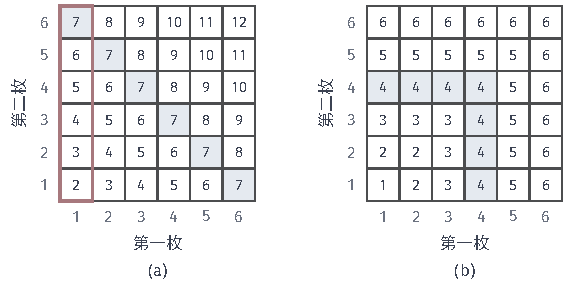
\includegraphics[width=96mm]{figures/07-probability/02-measure-theoretic-probability/tikz/pspace-dice-partitions/figure.pdf}
  \caption{同一个样本空间上的两种记录。每个格子是一个有序结果$(i,j)$。(a)格内是点数和$S$，浅蓝格子组成$\{S=7\}$；红框是事件“第一枚是$1$”，它把$S$取值相同的格子拆开了，只知道$S$无法判断它是否发生。(b)格内是较大点数$M$，浅蓝的L形区域是$\{M=4\}$。}
  \label{fig:pspace-dice-partitions}
\end{BookInlineFigure}

三种情形的共同点是：样本空间$\Omega$回答“可能出现哪些结果”，另需一个子集族回答“可以对哪些结果集合问概率”。前者是试验的描述，后者是我们愿意且能够提问的范围。

\paragraph{事件族应满足的运算}
什么样的子集族适合做事件族？从提问的角度看，至少有三条要求。整个$\Omega$应当是事件，“某个结果出现了”总能回答。若能判断$A$是否发生，也就能判断$A$不发生，所以事件族对补集封闭。若能逐一判断$A_1,A_2,\dots$是否发生，就应当能判断“其中至少一个发生”，所以事件族对可数并封闭。

为什么要求可数并而不只是有限并？第~\ref{chap:classical-probability}章抛硬币直到出现正面，事件“迟早出现正面”是“第$k$次首次出现正面”对$k=1,2,\dots$之并；有理数集是可数个单点之并。概率论中的极限陈述，例如“平均值收敛”，也都要用可数次并与交写出来。只要求有限并的事件族装不下这些事件。

这三条恰好是卷四$\sigma$代数的定义。设$\mathcal{F}$是$\Omega$的子集族，满足：
\begin{enumerate}
  \item $\Omega\in\mathcal{F}$；
  \item 若$A\in\mathcal{F}$，则$A^{\mathrm{c}}\in\mathcal{F}$；
  \item 若$A_1,A_2,\dots\in\mathcal{F}$，则$\bigcup_{k}A_k\in\mathcal{F}$。
\end{enumerate}
称$\mathcal{F}$为$\Omega$上的$\sigma$代数，$(\Omega,\mathcal{F})$为可测空间。由补集和可数并还能得到可数交：
\[
  \bigcap_{k}A_k=\Bigl(\bigcup_{k}A_k^{\mathrm{c}}\Bigr)^{\mathrm{c}}\in\mathcal{F},
\]
以及$\varnothing=\Omega^{\mathrm{c}}\in\mathcal{F}$、差集$A\setminus B=A\cap B^{\mathrm{c}}\in\mathcal{F}$。

\begin{definition}[事件]
\label{def:pspace-event}
设$(\Omega,\mathcal{F})$是可测空间。$\mathcal{F}$中的集合称为事件，$\mathcal{F}$称为\term{事件族}（family of events）。
\end{definition}

从此“事件”是一个相对于$\mathcal{F}$的概念。$\Omega$的子集未必是事件；同一个$\Omega$配上不同的$\mathcal{F}$，描述的是同一组结果上不同的提问范围。第一部分在有限或可数的$\Omega$上取全部子集，在实轴上只对区间及其有限并谈概率，都是这里的特例或其中的一部分。

\paragraph{有限样本空间上的事件族}
$\Omega$有限时，$\sigma$代数有一个具体的样子：它把$\Omega$分成若干块，事件恰好是若干块的并。块的构造是取包含某个点的所有事件之交。对$\omega\in\Omega$，令
\begin{equation}
  A(\omega)=\bigcap\{A\in\mathcal{F}:\omega\in A\},
  \label{eq:pspace-atom}
\end{equation}
称为$\omega$所在的\term{原子}（atom）。$\mathcal{F}$是有限族，所以这是有限交，$A(\omega)\in\mathcal{F}$。它是包含$\omega$的最小事件。

\begin{lemma}[有限样本空间上的$\sigma$代数]
\label{lem:pspace-finite-atoms}
设$\Omega$有限，$\mathcal{F}$是$\Omega$上的$\sigma$代数。则不同的原子两两不交，它们构成$\Omega$的一个划分；$\mathcal{F}$中每个事件都是若干个原子之并。若原子共有$k$个，则$\mathcal{F}$恰有$2^{k}$个事件。
\end{lemma}

\begin{proof}
先证两个原子要么相同、要么不交。设$A(\omega)\cap A(\omega')\neq\varnothing$。若$\omega\notin A(\omega')$，则$A(\omega)\setminus A(\omega')$是包含$\omega$的事件，且比$A(\omega)$小，与$A(\omega)$的最小性矛盾。所以$\omega\in A(\omega')$，于是$A(\omega)\subseteq A(\omega')$。对称地$A(\omega')\subseteq A(\omega)$，两者相同。

再证每个事件是原子之并。设$A\in\mathcal{F}$。对每个$\omega\in A$，$A$是包含$\omega$的事件，所以$A(\omega)\subseteq A$。于是
\[
  A=\bigcup_{\omega\in A}A(\omega),
\]
右边是若干个原子之并。反过来，原子都是事件，有限个事件之并仍是事件。所以$\mathcal{F}$恰由原子的各种并组成。$k$个两两不交的原子，每个选或不选，给出$2^{k}$个不同的并。
\end{proof}

在骰子的例子里，只知道$S$的观察者能判断的事件族，以$S$的$11$个取值对应的格子组为原子，即图~\ref{fig:pspace-dice-partitions}(a)中的各条反对角线。由引理~\ref{lem:pspace-finite-atoms}，这个事件族有$2^{11}=2048$个事件，而$36$个结果的全部子集有$2^{36}$个。“第一枚是$1$”不是原子之并，所以不在其中。只知道较大点数$M$的观察者，原子是图~\ref{fig:pspace-dice-partitions}(b)中的$6$个L形区域，事件族有$2^{6}=64$个事件。

\paragraph{生成的事件族}
实际建模时，我们通常只知道几个“想问的事件”，并不想逐一列出整个$\sigma$代数。卷四给出了办法：对$\Omega$的任意子集族$\mathcal{C}$，包含$\mathcal{C}$的所有$\sigma$代数之交仍是$\sigma$代数，它是包含$\mathcal{C}$的最小$\sigma$代数，记作$\sigma(\mathcal{C})$。它就是从$\mathcal{C}$出发、反复做补集与可数并所能得到的全部事件。

最简单的情形是一个事件$A$。包含$A$的$\sigma$代数必须含有$\Omega$、$A$和$A^{\mathrm{c}}$，因而含有$\varnothing$，而这四个集合已经对补集和并封闭，所以
\[
  \sigma(\{A\})=\{\varnothing,A,A^{\mathrm{c}},\Omega\}.
\]
两个相交的事件$A,B$把$\Omega$切成四块（图~\ref{fig:pspace-generated-events}）。四块都要在$\sigma(\{A,B\})$中，而它们的各种并已经构成$\sigma$代数，所以$\sigma(\{A,B\})$恰有$2^{4}=16$个事件。

\begin{BookInlineFigure}
  \centering
  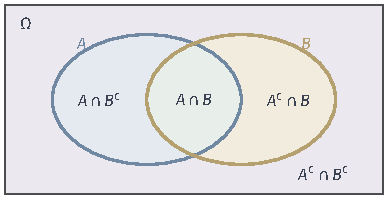
\includegraphics[width=66mm]{figures/07-probability/02-measure-theoretic-probability/tikz/pspace-generated-events/figure.pdf}
  \caption{两个事件$A$（蓝框）与$B$（黄框）把$\Omega$切成四个原子：$A\cap B^{\mathrm{c}}$（浅蓝）、$A\cap B$（浅绿）、$A^{\mathrm{c}}\cap B$（浅黄）和$A^{\mathrm{c}}\cap B^{\mathrm{c}}$（浅紫）。$\sigma(\{A,B\})$由这四块的全部$16$种并组成。}
  \label{fig:pspace-generated-events}
\end{BookInlineFigure}

对木棍上的随机点，想问的事件是区间。由区间生成的$\sigma$代数就是卷四的Borel $\sigma$代数，记作$\mathcal{B}([0,1))$。它不仅含有区间，还含有单点$\{x\}=\bigcap_n[x,x+1/n)$、有理数集、无理数集以及Cantor集等用可数次运算得到的集合。我们无法把它的成员一一列出，但对每个具体的集合，只要说出它怎样由区间经可数次运算得到，就知道它是事件。实轴上的$\mathcal{B}(\mathbb{R})$、$d$维空间上的$\mathcal{B}(\mathbb{R}^{d})$同理，它们也可以分别由半直线$(-\infty,x]$、左下象限$(-\infty,x_1]\times\cdots\times(-\infty,x_d]$生成。

表~\ref{tab:pspace-event-families}汇总了本章常用模型的样本空间与事件族。

\begin{BookInlineTable}
  \centering
  \caption{常用模型的样本空间与事件族}
  \label{tab:pspace-event-families}
  \begin{tabular}{lll}
    \toprule
    模型 & 样本空间$\Omega$ & 事件族$\mathcal{F}$ \\
    \midrule
    两枚骰子 & $36$个有序对 & 全部子集 \\
    只知道点数和 & $36$个有序对 & $\sigma(S)$，$2^{11}$个事件 \\
    木棍上的点 & $[0,1)$ & $\mathcal{B}([0,1))$ \\
    等待时间$W$ & $\mathbb{R}$ & $\mathcal{B}(\mathbb{R})$ \\
    \bottomrule
  \end{tabular}
\end{BookInlineTable}

表中的$\sigma(S)$是由点数和生成的事件族，第~\ref{sec:pspace-random-objects}节对一般的观测给出它的定义。

\section{概率测度}
\label{sec:pspace-measures}

事件族确定以后，要给每个事件指定一个概率。第~\ref{chap:classical-probability}章已经列出了三条要求：概率非负，必然事件的概率为$1$，互斥事件的概率相加。那一章的末尾还看到，抛硬币直到出现正面时，可加性必须对可数多个互斥事件成立，各次首次出现正面的概率$2^{-k}$加起来才等于$1$。把这些要求放在一起，概率就是卷四中总质量为一的测度。

\begin{definition}[概率测度与概率空间]
\label{def:pspace-probability-space}
设$(\Omega,\mathcal{F})$是可测空间。函数$\mathbb{P}:\mathcal{F}\to[0,1]$若满足$\mathbb{P}(\Omega)=1$，并且对任意两两不交的事件$A_1,A_2,\dots$有
\begin{equation}
  \mathbb{P}\Bigl(\bigcup_{k=1}^{\infty}A_k\Bigr)=\sum_{k=1}^{\infty}\mathbb{P}(A_k),
  \label{eq:pspace-countable-additivity}
\end{equation}
则称$\mathbb{P}$为\term{概率测度}（probability measure），称$(\Omega,\mathcal{F},\mathbb{P})$为\term{概率空间}（probability space）。
\end{definition}

式~\eqref{eq:pspace-countable-additivity}称为可数可加性。取$A_k=\varnothing$（$k>n$）就得到有限可加性，所以第一部分使用的规则都保留下来：补事件的概率$\mathbb{P}(A^{\mathrm{c}})=1-\mathbb{P}(A)$；单调性，即$A\subseteq B$时$\mathbb{P}(A)\leq\mathbb{P}(B)$；以及联合界
\[
  \mathbb{P}\Bigl(\bigcup_kA_k\Bigr)\leq\sum_k\mathbb{P}(A_k),
\]
它对可数个事件也成立。这些都是卷四测度基本性质的特例。

把概率看成单位质量的分配，可数可加性说的是：把一块区域切成可数多块，各块质量之和等于整块的质量。它不允许质量在“切成无穷多块”的过程中凭空出现或消失。下面先看这条要求带来的第一个后果。

\paragraph{概率的连续性}
事件常常由一列事件逼近：$\{W\leq1/n\}$随$n$增大而缩小，极限是$\{W\leq0\}$；“前$n$次中出现过正面”随$n$增大而扩大，极限是“迟早出现正面”。概率是否随事件一起取极限？

\begin{theorem}[概率的连续性]
\label{thm:pspace-continuity}
设$(\Omega,\mathcal{F},\mathbb{P})$是概率空间。
\begin{enumerate}
  \item 若$A_1\subseteq A_2\subseteq\cdots$，令$A=\bigcup_nA_n$，则
  \begin{equation}
    \mathbb{P}(A)=\lim_{n\to\infty}\mathbb{P}(A_n);
    \label{eq:pspace-continuity-up}
  \end{equation}
  \item 若$B_1\supseteq B_2\supseteq\cdots$，令$B=\bigcap_nB_n$，则
  \begin{equation}
    \mathbb{P}(B)=\lim_{n\to\infty}\mathbb{P}(B_n).
    \label{eq:pspace-continuity-down}
  \end{equation}
\end{enumerate}
\end{theorem}

\begin{proof}
先证递增的情形。把$A$切成互不相交的“新增部分”：令$C_1=A_1$，$C_k=A_k\setminus A_{k-1}$（$k\geq2$）。各$C_k$两两不交，且
\[
  A_n=\bigcup_{k=1}^{n}C_k,\qquad A=\bigcup_{k=1}^{\infty}C_k .
\]
由可数可加性与有限可加性，
\[
  \mathbb{P}(A)=\sum_{k=1}^{\infty}\mathbb{P}(C_k)=\lim_{n\to\infty}\sum_{k=1}^{n}\mathbb{P}(C_k)=\lim_{n\to\infty}\mathbb{P}(A_n).
\]

递减的情形取补集。$B_n^{\mathrm{c}}$递增，并集是$B^{\mathrm{c}}$，由第一部分，
\[
  1-\mathbb{P}(B)=\mathbb{P}(B^{\mathrm{c}})=\lim_{n\to\infty}\mathbb{P}(B_n^{\mathrm{c}})=1-\lim_{n\to\infty}\mathbb{P}(B_n).
\]
两边消去$1$即得式~\eqref{eq:pspace-continuity-down}。
\end{proof}

证明中递减情形用到了$\mathbb{P}(\Omega)=1$有限。对一般的测度，递减情形需要$B_1$的测度有限，例如实轴上的$[n,\infty)$递减到空集，长度却一直是无穷。概率测度总质量为一，这个条件自动满足。反过来，若一个集函数有限可加，又满足式~\eqref{eq:pspace-continuity-up}，取$A_n=C_1\cup\cdots\cup C_n$即可推出可数可加性。所以对有限可加的概率，“可数可加”与“沿递增序列连续”是同一个要求。

\paragraph{分布函数的性质}
连续性的第一个用途是补上第~\ref{chap:random-variables}章留下的证明：分布函数的基本性质对一般分布都成立。那里的分布是实轴上的概率，这里设$P$是$(\mathbb{R},\mathcal{B}(\mathbb{R}))$上的任一概率测度，令
\begin{equation}
  F(x)=P\bigl((-\infty,x]\bigr),\qquad x\in\mathbb{R}.
  \label{eq:pspace-cdf}
\end{equation}

$F$单调不减，因为$x<y$时$(-\infty,x]\subseteq(-\infty,y]$。对右连续性，取$x_n\downarrow x$，则$(-\infty,x_n]$递减，交集为$(-\infty,x]$，由式~\eqref{eq:pspace-continuity-down}得$F(x_n)\to F(x)$。同理，$(-\infty,-n]$递减到空集，$(-\infty,n]$递增到$\mathbb{R}$，所以
\[
  \lim_{x\to-\infty}F(x)=0,\qquad \lim_{x\to+\infty}F(x)=1 .
\]

左极限也有明确含义。取$x_n\uparrow x$且$x_n<x$，区间$(-\infty,x_n]$递增，并集是$(-\infty,x)$，于是
\[
  F(x^{-})=\lim_{n\to\infty}F(x_n)=P\bigl((-\infty,x)\bigr),
\]
跳跃高度$F(x)-F(x^{-})=P(\{x\})$正是单点的概率。这几步在第一部分只对概率表和密度验证过，现在对任何概率测度都成立，因为它们只用到可数可加性。

用等待时间$W$看一看这两个方向的极限。$W$的分布是
\begin{equation}
  P_W(A)=0.3\cdot\mathbf{1}_{A}(0)+0.7\int_{A\cap(0,\infty)}\mathrm{e}^{-t}\,\mathrm{d}t,\qquad A\in\mathcal{B}(\mathbb{R}),
  \label{eq:pspace-waiting-law}
\end{equation}
它的分布函数在$t\geq0$时为$F_W(t)=0.3+0.7(1-\mathrm{e}^{-t})$。从右侧逼近$0$，四个值是
\[
  F_W(1)\approx0.7425,\quad F_W(\tfrac12)\approx0.5754,\quad F_W(\tfrac14)\approx0.4548,\quad F_W(\tfrac18)\approx0.3823,
\]
它们递减到$F_W(0)=0.3$。从左侧逼近，$F_W(-1/n)=0$，极限是$P_W((-\infty,0))=0$。两侧极限之差$0.3$就是$P_W(\{0\})$，见图~\ref{fig:pspace-continuity}。

\begin{BookInlineFigure}
  \centering
  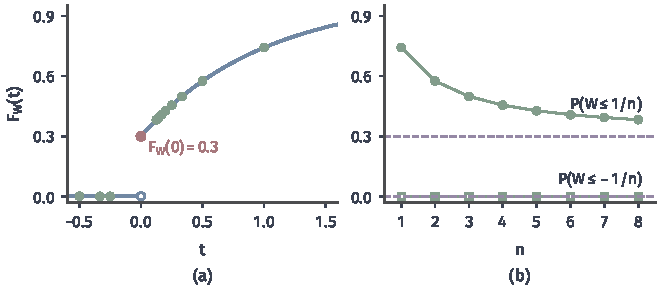
\includegraphics[width=112mm]{figures/07-probability/02-measure-theoretic-probability/matplotlib/pspace-continuity/figure.pdf}
  \caption{等待时间$W$的分布函数与概率的连续性。(a)蓝线是$F_W$，空心点是$0$处的左极限，红点是$F_W(0)=0.3$；右侧绿点是$t=1/n$处的值，左侧绿点是$t=-1/n$处的值。(b)绿色实心点是递减事件$\{W\leq1/n\}$的概率，趋于$0.3$；空心方块是递增事件$\{W\leq-1/n\}$的概率，恒为$0$。紫色虚线是两个极限。}
  \label{fig:pspace-continuity}
\end{BookInlineFigure}

\paragraph{已有模型怎样成为概率空间}
第一部分的每个模型都可以写成一个概率空间，只是事件族和概率的给法不同。

古典模型取$\Omega$有限，$\mathcal{F}$为全部子集，$\mathbb{P}(A)=\lvert A\rvert/\lvert\Omega\rvert$。有限个集合不可能有无穷多个两两不交的非空成员，可数可加性归结为有限可加性，也就是计数的加法。

概率表取$\Omega$可数，$\mathcal{F}$为全部子集，给每个$\omega$一个$p(\omega)\geq0$，且$\sum_{\omega}p(\omega)=1$，令$\mathbb{P}(A)=\sum_{\omega\in A}p(\omega)$。对两两不交的$A_1,A_2,\dots$，
\[
  \mathbb{P}\Bigl(\bigcup_{k}A_k\Bigr)=\sum_{k}\sum_{\omega\in A_k}p(\omega)=\sum_{k}\mathbb{P}(A_k),
\]
第一个等号把并集中的点按所属的$A_k$分组。非负项级数可以任意重排、分组而和不变，这就是可数可加性。

密度模型取$\Omega=\mathbb{R}$，$\mathcal{F}=\mathcal{B}(\mathbb{R})$。给定非负Borel函数$f$且$\int_{\mathbb{R}}f\,\mathrm{d}\lambda=1$，其中$\lambda$是Lebesgue测度，令
\begin{equation}
  \mathbb{P}(A)=\int_{A}f\,\mathrm{d}\lambda,\qquad A\in\mathcal{B}(\mathbb{R}).
  \label{eq:pspace-density-model}
\end{equation}
对两两不交的$A_k$，被积函数可以逐项拆开：
\[
  \mathbf{1}_{\bigcup_kA_k}f=\sum_k\mathbf{1}_{A_k}f,
\]
右边的部分和是递增的非负函数列。由单调收敛定理，积分与求和可以交换，于是式~\eqref{eq:pspace-density-model}可数可加。在区间上，这个积分与第一部分的黎曼积分（含反常积分）一致，可参考\BookChapterRef{chap:integration}{卷四第6章“积分”}。

混合模型把两者相加。式~\eqref{eq:pspace-waiting-law}中，$A\mapsto\mathbf{1}_{A}(0)$是$0$处的单点测度，第二项是密度为$\mathrm{e}^{-t}\mathbf{1}_{\{t>0\}}$的测度。非负系数的测度之和仍是测度，总质量$0.3+0.7=1$，所以$P_W$是概率测度。单点$\{0\}$和各种区间在同一个$\mathcal{B}(\mathbb{R})$中，可以一起运算。

\paragraph{由分布函数给出的模型}
Cantor分布既没有概率表也没有密度，它只有分布函数。第~\ref{chap:random-variables}章说过，满足三条性质的函数都可以用来规定模型；现在可以说清这句话的含义。

\begin{theorem}[分布函数确定实轴上的概率]
\label{thm:pspace-cdf-measure}
设$F:\mathbb{R}\to[0,1]$单调不减、右连续，且$\lim_{x\to-\infty}F(x)=0$，$\lim_{x\to+\infty}F(x)=1$。则$(\mathbb{R},\mathcal{B}(\mathbb{R}))$上存在唯一的概率测度$P$，使得
\begin{equation}
  P\bigl((-\infty,x]\bigr)=F(x),\qquad x\in\mathbb{R}.
  \label{eq:pspace-cdf-measure}
\end{equation}
\end{theorem}

\begin{proof}
存在性就是卷四的Stieltjes测度定理：对单调不减、右连续的$F$，存在$\mathcal{B}(\mathbb{R})$上的测度$P$，使$P((a,b])=F(b)-F(a)$对一切$a<b$成立。令$a\to-\infty$，由连续性得
\[
  P\bigl((-\infty,b]\bigr)=\lim_{a\to-\infty}\bigl(F(b)-F(a)\bigr)=F(b).
\]
再令$b\to+\infty$得$P(\mathbb{R})=1$。

唯一性用卷四的$\pi$--$\lambda$定理。半直线族$\{(-\infty,x]:x\in\mathbb{R}\}$对有限交封闭，因为$(-\infty,x]\cap(-\infty,y]=(-\infty,\min\{x,y\}]$，所以它是$\pi$系统，并且生成$\mathcal{B}(\mathbb{R})$。两个概率测度若在一个生成$\sigma$代数的$\pi$系统上一致，就在整个$\sigma$代数上一致。满足式~\eqref{eq:pspace-cdf-measure}的两个概率测度在半直线上一致，因此相同。
\end{proof}

这个定理有两层意思。唯一性说，分布函数记录了实轴上全部Borel集的概率，而不只是区间的概率；第一部分只能从$F$读出区间的概率，现在知道其余集合的概率也已被确定。存在性说，Cantor函数确实对应一个概率测度，第~\ref{chap:random-variables}章的Cantor分布不是一个只有分布函数的“形式对象”。

\paragraph{单点的概率与总概率}
木棍上的均匀随机点由$\Omega=[0,1)$、$\mathcal{F}=\mathcal{B}([0,1))$和长度测度$\lambda$给出。每个单点的概率为零：对任意$h>0$，$\{x\}\subseteq[x,x+h)$，所以$\lambda(\{x\})\leq h$，再令$h\to0$。由可数可加性，任何可数集的概率也为零，特别地
\[
  \mathbb{P}\bigl(\mathbb{Q}\cap[0,1)\bigr)=\sum_{q}\lambda(\{q\})=0 .
\]

不借助单点的结论，也可以直接看到有理数集“太稀”。把有理数排成一列$q_1,q_2,\dots$，用以$q_k$为中心、长$\varepsilon/2^{k}$的区间覆盖它，总长度不超过$\varepsilon$（图~\ref{fig:pspace-rational-cover}）。$\varepsilon$可以任意小，所以有理数集的概率为零，尽管有理数在$[0,1)$中处处稠密。

\begin{BookInlineFigure}
  \centering
  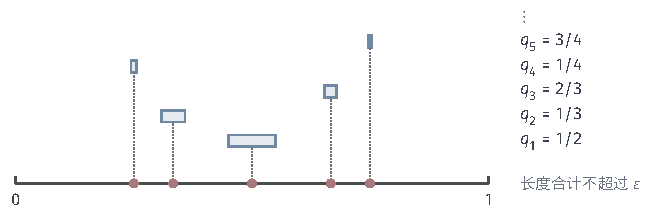
\includegraphics[width=104mm]{figures/07-probability/02-measure-theoretic-probability/tikz/pspace-rational-cover/figure.pdf}
  \caption{用总长度不超过$\varepsilon$的区间覆盖$[0,1)$中的有理数，这里$\varepsilon=0.2$。红点是按某种次序排列的前五个有理数$q_k$，浅蓝区间以$q_k$为中心，长$\varepsilon/2^{k}$，依次为$0.1,0.05,0.025,\dots$，越来越短。}
  \label{fig:pspace-rational-cover}
\end{BookInlineFigure}

另一方面，$[0,1)$是它的单点之并，每个单点的概率都是$0$，总概率却是$1$。这并不矛盾。可数可加性只对可数个事件成立，而$[0,1)$的点不可数。若硬要对不可数个零相加，把和定义为所有有限部分和的上确界，结果是$0$而不是$1$。所以“总概率等于各点概率之和”只在可数情形成立。

质量的比喻能帮助理解这一点。一根质量为$1$、均匀的细棒，任何一点处都没有质量，质量只存在于有长度的小段上；密度描述的是单位长度上的质量，而不是某个点的质量。概率表适合把质量集中在可数个点上的模型，长度测度与密度适合把质量连续铺开的模型，$W$的分布兼有两者。概率测度的语言不偏向任何一种：它只规定事件的概率，并要求对可数个不交事件可加。

\subsection{零概率与几乎必然}
\label{sec:pspace-null-events}

在古典模型中，若每个样本点的概率都为正，那么概率为零的事件只有空集。连续模型打破了这一点：$\{U=1/2\}$非空，$U$完全可能落在$1/2$，可它的概率是$0$。需要一套说法，既承认这些事件可能发生，又在计算中把它们略去。

\begin{definition}[零概率事件与几乎必然]
\label{def:pspace-almost-sure}
设$(\Omega,\mathcal{F},\mathbb{P})$是概率空间。满足$\mathbb{P}(N)=0$的事件$N$称为\term{零概率事件}（null event）。若一个关于样本点的陈述不成立的点全体包含于某个零概率事件，则称该陈述\term{几乎必然}（almost surely）成立，简记为a.s.。
\end{definition}

这就是卷四“几乎处处”在概率测度下的说法。定义只要求失败点集\emph{包含于}一个零概率事件，因为失败点集本身未必在$\mathcal{F}$中；下一小节的完备化讨论这种情形。等价地，若陈述成立的点集是事件，几乎必然成立就是它的概率等于$1$。

\paragraph{不可能与零概率}
空集是不可能事件，它在任何结果下都不发生。零概率事件可以发生，只是在概率的计算中不占质量。$U$是均匀随机点，$\{U=1/2\}$、$\{U\in\mathbb{Q}\}$都是非空的零概率事件，相应地，“$U\neq1/2$”“$U$是无理数”都几乎必然成立，但不是必然成立。等待时间的例子中，$\{W=1\}$概率为零，$\{W=0\}$的概率却是$0.3$；哪些单点是零概率事件，由概率测度决定，与样本点本身无关。

零概率事件还依赖于所用的概率。在$\Omega=\{0,1\}$上，若$\mathbb{P}(\{1\})=0$，“结果是$0$”几乎必然成立；换成$\mathbb{P}(\{1\})=1/2$，同一句话就不成立了。所以说“几乎必然”时，必须清楚是相对于哪个概率测度。

\paragraph{可数个几乎必然的陈述}
几乎必然的陈述可以放心地合并可数次，这是它最常用的性质。

\begin{lemma}[可数个零概率事件之并]
\label{lem:pspace-countable-null}
若$N_1,N_2,\dots$都是零概率事件，则$\bigcup_kN_k$也是零概率事件。因此，可数个各自几乎必然成立的陈述，同时几乎必然成立。
\end{lemma}

\begin{proof}
由联合界，
\[
  0\leq\mathbb{P}\Bigl(\bigcup_{k}N_k\Bigr)\leq\sum_{k}\mathbb{P}(N_k)=0 .
\]
设第$k$个陈述在零概率事件$N_k$之外成立，则所有陈述在$\bigcup_kN_k$之外同时成立，而这个并集概率为零。
\end{proof}

第一个例子补上第~\ref{chap:random-vectors}章留下的一步。设$Y$与$L$是同一样本空间上的两个函数，已知对每个$\varepsilon>0$都有$\mathbb{P}(\lvert Y-L\rvert>\varepsilon)=0$。$Y$与$L$不相等，当且仅当它们相差某个$1/n$以上，所以
\[
  \{Y\neq L\}=\bigcup_{n=1}^{\infty}\bigl\{\lvert Y-L\rvert>1/n\bigr\}.
\]
右边是可数个零概率事件之并，由引理~\ref{lem:pspace-countable-null}，$\mathbb{P}(Y\neq L)=0$，即$\mathbb{P}(Y=L)=1$。这里只取$\varepsilon=1/n$这可数个值就够了，不需要对每个正数$\varepsilon$分别处理。

\paragraph{不可数个例外}
可数性不能省略。设$U$是均匀随机点，对每个$t\in[0,1)$令
\[
  X_t(\omega)=\mathbf{1}_{\{U(\omega)=t\}},
\]
即$U$恰好等于$t$时取$1$，否则取$0$。对每个固定的$t$，$X_t\neq0$的事件是$\{U=t\}$，概率为零，所以$X_t=0$几乎必然成立。

可是对每个样本点$\omega$，取$t=U(\omega)$就有$X_t(\omega)=1$。于是
\[
  \bigl\{\omega:\ X_t(\omega)=0\text{ 对一切 }t\text{ 成立}\bigr\}=\varnothing .
\]
“对每个$t$，几乎必然$X_t=0$”成立，“几乎必然对一切$t$都有$X_t=0$”却完全不成立。原因是例外事件$\{U=t\}$随$t$变化，不可数个零概率事件之并是整个$\Omega$。图~\ref{fig:pspace-uncountable-spikes}画出了三个样本点对应的函数$t\mapsto X_t(\omega)$：每条都只在一个位置有尖峰，固定任何一个时刻$t_0$去看，几乎看不到尖峰；但每条曲线都有尖峰。

\begin{BookInlineFigure}
  \centering
  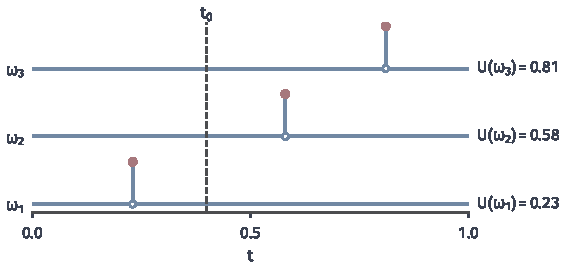
\includegraphics[width=96mm]{figures/07-probability/02-measure-theoretic-probability/matplotlib/pspace-uncountable-spikes/figure.pdf}
  \caption{$X_t=\mathbf{1}_{\{U=t\}}$在三个样本点上的取值，横轴是$t$。每条蓝线只在$t=U(\omega)$处跳到$1$（红点）。虚线是固定时刻$t_0$，它碰到尖峰的概率为零；然而每个样本点的曲线都有一个尖峰。}
  \label{fig:pspace-uncountable-spikes}
\end{BookInlineFigure}

要从“每个$t$几乎必然”推出“几乎必然对一切$t$”，需要额外的结构。例如，若已知每条曲线$t\mapsto X_t(\omega)$都连续，就只需检查可数个有理数时刻：它们在零概率事件之外同时为零，连续性再把结论推到所有$t$。上面的$X_t$不连续，这条路走不通。以连续时间为指标的随机对象经常遇到这个问题，本章只处理可数个陈述。

\subsection{完备化}
\label{sec:pspace-completion}

几乎必然的陈述允许在零概率事件上随意修改。修改以后的对象还在原来的事件族里吗？先看一个小例子。

\paragraph{修改可能破坏可测性}
取$\Omega=\{1,2,3\}$，事件族与概率为
\[
  \mathcal{F}=\bigl\{\varnothing,\{1\},\{2,3\},\Omega\bigr\},\qquad \mathbb{P}(\{1\})=1,\quad \mathbb{P}(\{2,3\})=0 .
\]这个事件族只能区分“结果是$1$”与“结果在$\{2,3\}$中”。按卷四的说法，函数$X:\Omega\to\mathbb{R}$\emph{可测}是指对每个Borel集$B$，$\{X\in B\}\in\mathcal{F}$；第~\ref{sec:pspace-random-objects}节将把这样的函数称为随机变量。

$X\equiv0$可测，因为它的每个原像都是$\varnothing$或$\Omega$。令$X'=\mathbf{1}_{\{2\}}$，它与$X$只在点$2$不同，而$\{2\}\subseteq\{2,3\}$包含于零概率事件，所以$X'=X$几乎必然成立。然而$\{X'=1\}=\{2\}\notin\mathcal{F}$，$X'$不可测。两个函数几乎必然相等，一个可测、一个不可测，问题出在$\mathcal{F}$不含零概率事件$\{2,3\}$的子集。

\paragraph{完备化的定义}
卷四的完备化正好补上这些集合。称概率空间$(\Omega,\mathcal{F},\mathbb{P})$\term{完备概率空间}（complete probability space），若每个零概率事件的每个子集都属于$\mathcal{F}$。对任意概率空间，令
\begin{equation}
  \overline{\mathcal{F}}=\{A\cup M:\ A\in\mathcal{F},\ M\subseteq N\text{ 对某个零概率事件 }N\},\qquad \overline{\mathbb{P}}(A\cup M)=\mathbb{P}(A).
  \label{eq:pspace-completion}
\end{equation}
卷四证明了：$\overline{\mathcal{F}}$是包含$\mathcal{F}$的$\sigma$代数，$\overline{\mathbb{P}}$与表示方式无关，是$\overline{\mathcal{F}}$上的概率测度，在$\mathcal{F}$上与$\mathbb{P}$一致，并且$(\Omega,\overline{\mathcal{F}},\overline{\mathbb{P}})$完备。

在上面的例子中，零概率事件只有$\varnothing$和$\{2,3\}$，它们的子集$\{2\}$、$\{3\}$被补入，再与$\{1\}$取并，得到全部$8$个子集（图~\ref{fig:pspace-completion}）。新补入的事件中，含点$1$的概率为$1$，不含点$1$的概率为$0$；原有$4$个事件的概率不变。

\begin{BookInlineFigure}
  \centering
  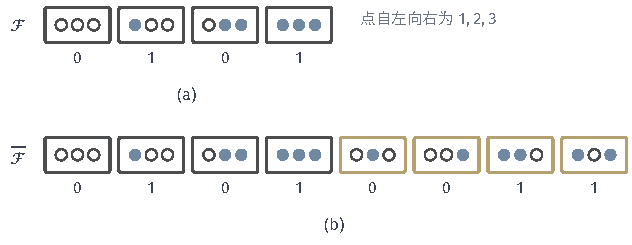
\includegraphics[width=107mm]{figures/07-probability/02-measure-theoretic-probability/tikz/pspace-completion/figure.pdf}
  \caption{三点样本空间的完备化。每个方框是一个事件，实心点表示该点属于事件，下方数字是概率。(a)原事件族$\mathcal{F}$只有$4$个事件；(b)完备化补入零概率事件$\{2,3\}$的子集及其与$\{1\}$的并（黄框），共$8$个事件，原有事件的概率不变。}
  \label{fig:pspace-completion}
\end{BookInlineFigure}

\paragraph{完备空间中的修改}
在完备的概率空间里，零概率事件上的修改不会破坏可测性。

\begin{theorem}[零概率修改保持可测性]
\label{thm:pspace-modification}
设$(\Omega,\mathcal{F},\mathbb{P})$完备，$X:\Omega\to\mathbb{R}$可测，$X':\Omega\to\mathbb{R}$满足：存在零概率事件$N$，使得在$N$之外$X'=X$。则$X'$可测，且对每个Borel集$B$，
\begin{equation}
  \mathbb{P}(X'\in B)=\mathbb{P}(X\in B).
  \label{eq:pspace-modification}
\end{equation}
\end{theorem}

\begin{proof}
把$\{X'\in B\}$按是否落在$N$中分成两块：
\[
  \{X'\in B\}=\bigl(\{X\in B\}\cap N^{\mathrm{c}}\bigr)\cup\bigl(\{X'\in B\}\cap N\bigr).
\]
在$N^{\mathrm{c}}$上$X'=X$，所以第一块等于$\{X\in B\}\cap N^{\mathrm{c}}$，它是两个事件之交，属于$\mathcal{F}$。第二块包含于零概率事件$N$，由完备性也属于$\mathcal{F}$，且概率为零。所以$\{X'\in B\}\in\mathcal{F}$，并且
\[
  \mathbb{P}(X'\in B)=\mathbb{P}\bigl(\{X\in B\}\cap N^{\mathrm{c}}\bigr)=\mathbb{P}(X\in B),
\]
最后一步是因为$\{X\in B\}$与$\{X\in B\}\cap N^{\mathrm{c}}$相差的部分包含于$N$。
\end{proof}

木棍上的随机点就有这样的例子。卷四指出，$\mathcal{B}([0,1))$关于长度的完备化是Lebesgue可测集族。Cantor集的长度为零，在完备化后它的每个子集都是事件，概率都是零，其中包括不是Borel集的子集。于是，把一个随机变量在Cantor集的任意子集上改掉，得到的函数在完备空间中仍然可测，所有概率都不变。

\paragraph{完备化不做的事}
完备化只是把“包含于零概率事件”的集合补进来并赋予概率零，它不改变原有事件的概率，也不会让任何零概率事件变成正概率事件。特别地，它不能帮助我们以零概率事件为条件。给定$U=1/2$时某事件的条件概率，按第~\ref{chap:classical-probability}章的定义是
\[
  \mathbb{P}(A\mid U=1/2)=\frac{\mathbb{P}(A\cap\{U=1/2\})}{\mathbb{P}(U=1/2)},
\]
分母为零，完备化前后都一样。给定连续观测值求条件规律，要用第~\ref{chap:conditional-expectation}章和第~\ref{chap:conditional-distributions}章的办法。

完备化也有代价。零概率事件依赖于概率测度，对一个测度完备的事件族，换一个测度就未必完备；同时讨论多个概率测度时，通常保留原来的事件族。对取值空间，惯例是使用Borel $\sigma$代数而不完备化：卷四说明过，Lebesgue可测函数与连续函数的复合未必Lebesgue可测，取值一侧若换成更大的事件族，复合运算就可能失去可测性。本章约定：样本空间一侧需要时可以完备化，取值空间一律使用Borel $\sigma$代数。

\section{随机对象}
\label{sec:pspace-random-objects}

第~\ref{chap:random-variables}章把随机变量定义为样本空间上的实值函数，并直接对$\{X\in B\}$谈概率。那时事件族是全部子集或者只涉及区间，$\{X\in B\}$是否为事件不成问题。现在事件族是指定的$\mathcal{F}$，一个函数的原像未必落在$\mathcal{F}$里；而我们还会观测向量、矩阵、图这样的对象。什么样的函数才配称为随机变量？

\paragraph{可测性：观测引出的问题都有概率}
回到只知道点数和的观察者，他的事件族是$\sigma(S)$。若他想研究第一枚骰子的点数$X_1$，就会遇到$\{X_1=1\}\notin\sigma(S)$：这个“随机变量”提出的问题，他的事件族无法回答。所以随机变量的定义必须保证，凡是由它引出的“取值落在某个集合中”的问题，答案都在事件族里。卷四的可测映射正是这个要求。

\begin{definition}[随机对象与随机变量]
\label{def:pspace-random-object}
设$(\Omega,\mathcal{F},\mathbb{P})$是概率空间，$(E,\mathcal{E})$是可测空间。映射$X:\Omega\to E$若满足
\begin{equation}
  X^{-1}(B)=\{\omega\in\Omega:X(\omega)\in B\}\in\mathcal{F},\qquad B\in\mathcal{E},
  \label{eq:pspace-measurable}
\end{equation}
则称$X$为取值于$E$的\term{随机对象}（random element）。取值于$(\mathbb{R},\mathcal{B}(\mathbb{R}))$的随机对象称为随机变量，取值于$(\mathbb{R}^{d},\mathcal{B}(\mathbb{R}^{d}))$的称为$d$维随机向量。
\end{definition}

图~\ref{fig:pspace-random-object-map}画出了这个定义。$X$把$\Omega$中的点送到$E$中；对$E$中的集合$B$，把所有被送进$B$的样本点收集起来，就是原像$X^{-1}(B)$。这个原像可以由几块分开的区域组成，可测性要求它是事件，从而有概率。

\begin{BookInlineFigure}
  \centering
  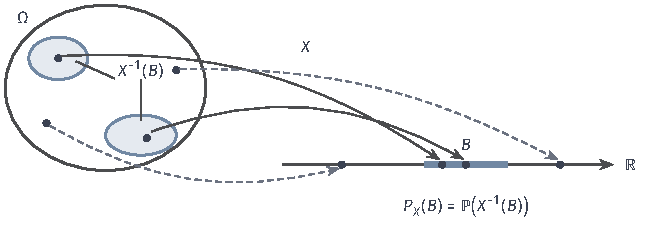
\includegraphics[width=110mm]{figures/07-probability/02-measure-theoretic-probability/tikz/pspace-random-object-map/figure.pdf}
  \caption{随机变量$X:\Omega\to\mathbb{R}$与原像。实线箭头把浅蓝的两块区域中的点送进集合$B$（粗蓝线段），虚线箭头把其他点送到$B$之外。$X^{-1}(B)$是两块区域之并，可测性要求它是事件，它的概率就是取值落在$B$中的概率。}
  \label{fig:pspace-random-object-map}
\end{BookInlineFigure}

定义要求对$\mathcal{E}$中\emph{每个}集合检查原像，实际操作时只需检查一个生成族。卷四的生成族判据说：若$\mathcal{E}=\sigma(\mathcal{C})$，则$X$可测当且仅当对每个$C\in\mathcal{C}$都有$X^{-1}(C)\in\mathcal{F}$。原因是原像运算与补集、可数并交换，使得原像为事件的集合$B$构成一个$\sigma$代数，它包含$\mathcal{C}$，也就包含$\sigma(\mathcal{C})$。对实值函数，取半直线为生成族，得到常用的判别：
\begin{equation}
  X\text{ 是随机变量}\iff\{X\leq x\}\in\mathcal{F}\quad\text{对一切 }x\in\mathbb{R}.
  \label{eq:pspace-rv-criterion}
\end{equation}

\paragraph{常见的取值空间}
映射$\bm{X}=(X_1,\dots,X_d):\Omega\to\mathbb{R}^{d}$是随机向量，当且仅当每个坐标$X_i$都是随机变量。一方面，坐标投影连续，因而Borel可测，可测映射的复合仍可测。另一方面，$\mathcal{B}(\mathbb{R}^{d})$由左下象限生成，而
\[
  \{\bm{X}\in(-\infty,x_1]\times\cdots\times(-\infty,x_d]\}=\bigcap_{i=1}^{d}\{X_i\leq x_i\}
\]
是$d$个事件之交。所以第~\ref{chap:random-vectors}章逐个坐标定义的随机向量，正好是这里的$\mathbb{R}^{d}$值随机对象。

随机矩阵可以看成拉直的向量。把$m\times n$实矩阵按元素排成$\mathbb{R}^{mn}$中的向量，$\mathbb{R}^{m\times n}$就带有Borel $\sigma$代数，随机矩阵$\bm{M}$可测当且仅当每个元素$M_{i,j}$都是随机变量。例如随机向量$\bm{X}$的外积$\bm{X}\bm{X}^{\top}$，其元素$X_iX_j$是随机变量的乘积，所以它是随机矩阵。

有限集合是另一类常见的取值空间，配上全部子集作为事件族。这时可测性只需检查单点：$X$可测当且仅当对每个可能的取值$g$，$\{X=g\}\in\mathcal{F}$，因为任何子集都是有限个单点之并。

\paragraph{有限随机图}
以$3$个带标号顶点上的随机图为例。$3$个顶点之间有$3$条可能的边，每条边出现与否用一个比特记录，样本空间是$\Omega=\{0,1\}^{3}$，取全部子集为事件族，并让$8$个结果等可能。映射$G$把结果$\omega=(e_{1,2},e_{1,3},e_{2,3})$送到边集为$\{\{i,j\}:e_{i,j}=1\}$的图。取值空间$E$是这$3$个顶点上全部$2^{3}=8$个图，同样取全部子集。

在这个模型里$\Omega$与$E$一一对应，可测性不成问题。值得注意的是由图算出的数值。边数$N=e_{1,2}+e_{1,3}+e_{2,3}$是$E$上函数与$G$的复合，它把$8$个图分成$4$组（图~\ref{fig:pspace-random-graph}），由此得到
\[
  \mathbb{P}(N=0)=\tfrac18,\quad \mathbb{P}(N=1)=\tfrac38,\quad \mathbb{P}(N=2)=\tfrac38,\quad \mathbb{P}(N=3)=\tfrac18 .
\]
“图是三角形”是事件$\{N=3\}$，“图连通”是$\{N\geq2\}$，因为$3$个顶点上的图连通当且仅当至少有$2$条边。

\begin{BookInlineFigure}
  \centering
  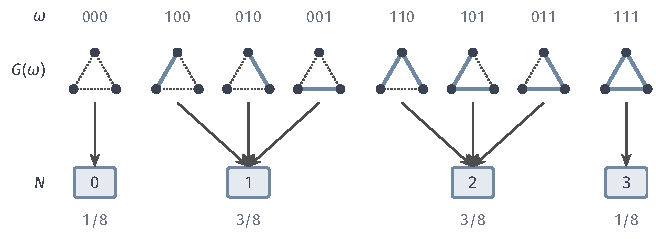
\includegraphics[width=111mm]{figures/07-probability/02-measure-theoretic-probability/tikz/pspace-random-graph/figure.pdf}
  \caption{$3$个顶点上的随机图。上行是结果$\omega=(e_{1,2},e_{1,3},e_{2,3})$，中间是对应的图$G(\omega)$，蓝色实线是出现的边，点线是未出现的边；顶点$1$在上，$2$在左下，$3$在右下。边数$N$把$8$个等可能的图分成$4$组，下方是各组的概率。}
  \label{fig:pspace-random-graph}
\end{BookInlineFigure}

更大的随机图也一样：$n$个顶点有$n(n-1)/2$条可能的边，取值空间有$2^{n(n-1)/2}$个图。边数、三角形个数、最大度数、是否连通，都是有限集合上的函数，与$G$复合后自动成为随机变量。一般地，若$X$是取值于$(E,\mathcal{E})$的随机对象，$g:E\to E'$是可测映射，则对$B\in\mathcal{E}'$，
\[
  (g\circ X)^{-1}(B)=X^{-1}\bigl(g^{-1}(B)\bigr)\in\mathcal{F},
\]
因为$g^{-1}(B)\in\mathcal{E}$。所以$g(X)$也是随机对象。连续函数关于Borel $\sigma$代数可测，于是随机向量的和、积、范数，随机对称矩阵的迹，都是随机变量。

\paragraph{观测生成的事件族}
可测性说明观测\emph{不超出}事件族的回答能力。反过来也可以问：一个观测本身能回答哪些问题？观测$X$之后，对每个$B\in\mathcal{E}$，我们都能判断$X\in B$是否成立，也就是判断事件$X^{-1}(B)$是否发生。这些事件收集起来，就是$X$提供的信息。

\begin{definition}[观测生成的$\sigma$代数]
\label{def:pspace-generated-sigma}
设$X:\Omega\to E$是取值于$(E,\mathcal{E})$的随机对象。称
\begin{equation}
  \sigma(X)=\bigl\{X^{-1}(B):\ B\in\mathcal{E}\bigr\}
  \label{eq:pspace-generated-sigma}
\end{equation}
为$X$\term{生成的$\sigma$代数}（$\sigma$-algebra generated by $X$）。对多个随机对象$X_1,\dots,X_n$，$\sigma(X_1,\dots,X_n)$指向量$(X_1,\dots,X_n)$生成的$\sigma$代数。
\end{definition}

$\sigma(X)$确实是$\sigma$代数：$X^{-1}(E)=\Omega$，并且原像与补集、可数并交换，
\[
  \bigl(X^{-1}(B)\bigr)^{\mathrm{c}}=X^{-1}(B^{\mathrm{c}}),\qquad \bigcup_{k}X^{-1}(B_k)=X^{-1}\Bigl(\bigcup_kB_k\Bigr).
\]
它包含于$\mathcal{F}$，这就是可测性。它也是使$X$可测的最小$\sigma$代数：任何使$X$可测的$\sigma$代数都必须含有全部原像$X^{-1}(B)$。

当$X$只取有限个值时，$\sigma(X)$的原子就是$X$的各个等值集$\{X=x\}$，事件是若干等值集之并。第~\ref{sec:pspace-events}节的“只知道点数和”就是$\sigma(S)$，它的原子是$11$条反对角线；“只知道较大点数”就是$\sigma(M)$，原子是$6$个L形区域。只知道“点数和是否为$7$”，对应的是指示变量$\mathbf{1}_{\{S=7\}}$，它生成的$\sigma$代数只有$4$个事件。

\paragraph{函数只会减少信息}
对观测结果再作变换，信息不会增加。设$g$可测，对$B\in\mathcal{E}'$，
\[
  \bigl(g(X)\bigr)^{-1}(B)=X^{-1}\bigl(g^{-1}(B)\bigr)\in\sigma(X),
\]
所以$\sigma(g(X))\subseteq\sigma(X)$。在骰子的例子里，$\mathbf{1}_{\{S=7\}}$是$S$的函数，$\sigma(\mathbf{1}_{\{S=7\}})\subseteq\sigma(S)$：知道点数和就知道它是否为$7$，反之不行。若$g$是双向可测的一一映射，两个方向都用上述包含关系，得到$\sigma(g(X))=\sigma(X)$：可逆的重新编码不改变信息。

木棍上的随机点给出一串逐渐精细的观测。设$\Omega=[0,1)$，$\omega$的二进制展开为$0.D_1D_2D_3\cdots$，取不以无穷个$1$结尾的那种展开，即
\[
  D_k(\omega)=\lfloor2^{k}\omega\rfloor-2\lfloor2^{k-1}\omega\rfloor\in\{0,1\}.
\]
记$K=\lfloor4\omega\rfloor$，它告诉我们$\omega$落在哪个四分之一区间。图~\ref{fig:pspace-nested-information}列出了几个观测的原子。$D_1=\lfloor K/2\rfloor$与$D_2=K-2D_1$都是$K$的函数，所以$\sigma(D_1)$和$\sigma(D_2)$都包含于$\sigma(K)$；$K$又是$\lfloor8\omega\rfloor$的函数。$\sigma(D_2)$的一个原子是$[1/4,1/2)\cup[3/4,1)$，由两段不相邻的区间组成，它说明粗信息未必是“把区间分得粗一点”。$\sigma(D_1)$与$\sigma(D_2)$互不包含，两者合起来恰好是$\sigma(K)$。

\begin{BookInlineFigure}
  \centering
  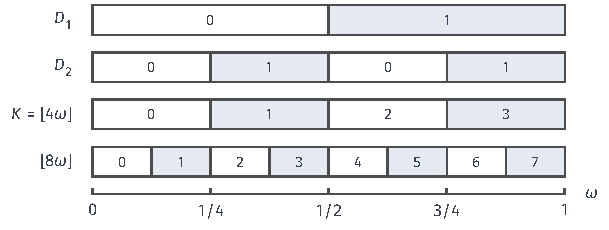
\includegraphics[width=103mm]{figures/07-probability/02-measure-theoretic-probability/tikz/pspace-nested-information/figure.pdf}
  \caption{$\Omega=[0,1)$上几个观测生成的原子。每一行把$[0,1)$分成若干格，格内数字是该观测的取值，浅蓝格子取奇数值。$D_1$、$D_2$是前两位二进制数字，$K=\lfloor4\omega\rfloor$。$\sigma(D_1)$与$\sigma(D_2)$都包含于$\sigma(K)$，$\sigma(K)$又包含于$\sigma(\lfloor8\omega\rfloor)$；$D_2$的原子各由两段不相邻的区间组成。}
  \label{fig:pspace-nested-information}
\end{BookInlineFigure}

观测$X(\omega)=\omega$本身生成全部Borel集，它提供完整的信息。这里讨论的都是一次观测，或同时取得的有限个观测。信息随时间逐步增加、后一时刻知道得比前一时刻多的情形，要用一列递增的$\sigma$代数描述，属于随机过程的内容。第~\ref{chap:conditional-expectation}章将以$\sigma(X)$为“已知信息”，研究给定信息后怎样求平均。

\section{分布与推前}
\label{sec:pspace-distributions}

随机变量是样本空间上的函数，可是多数问题只关心它的取值落在哪里、各处概率多大，并不关心是哪个样本点产生了这个取值。第~\ref{chap:random-variables}章把这种“取值的规律”称为分布，并只对区间及其有限并计算过它。现在把分布定义为取值空间上的一个完整的概率测度。

\paragraph{分布的定义}
随机对象$X$把每个样本点$\omega$送到$E$中的点$X(\omega)$。把$\omega$所带的概率质量随之搬过去，$E$中集合$B$所收到的质量，就是被送进$B$的那些样本点的质量之和，即$\mathbb{P}(X^{-1}(B))$。

\begin{definition}[分布]
\label{def:pspace-distribution}
设$X$是取值于$(E,\mathcal{E})$的随机对象。称
\begin{equation}
  P_X(B)=\mathbb{P}\bigl(X^{-1}(B)\bigr)=\mathbb{P}(X\in B),\qquad B\in\mathcal{E},
  \label{eq:pspace-distribution}
\end{equation}
为$X$的分布。$P_X$是$\mathbb{P}$在$X$下的推前测度，也记作$\mathbb{P}\circ X^{-1}$。
\end{definition}

$P_X$是$(E,\mathcal{E})$上的概率测度。总质量$P_X(E)=\mathbb{P}(\Omega)=1$；若$B_1,B_2,\dots$两两不交，它们的原像也两两不交，并且原像之并等于并集的原像，于是由$\mathbb{P}$的可数可加性，
\[
  P_X\Bigl(\bigcup_kB_k\Bigr)=\mathbb{P}\Bigl(\bigcup_kX^{-1}(B_k)\Bigr)=\sum_k\mathbb{P}\bigl(X^{-1}(B_k)\bigr)=\sum_kP_X(B_k).
\]
推前测度的一般理论，包括映射下的密度公式，可参考\BookChapterRef{chap:pushforward-measures}{卷四第9章“推前测度”}。

有了$P_X$，关于$X$取值的问题都可以在$(E,\mathcal{E},P_X)$上回答，不必再回到$\Omega$。第~\ref{chap:random-variables}章说“取值集合可以当作新的样本空间”，现在有了准确的含义：$(E,\mathcal{E},P_X)$本身就是一个概率空间。

\paragraph{用原像计算分布}
在木棍模型$\Omega=[0,1)$上定义$X(\omega)=-\ln(1-\omega)$。$X$连续且严格递增，从$0$增加到$+\infty$，因而是随机变量。对$x\geq0$，$X>x$等价于$\omega>1-\mathrm{e}^{-x}$，所以
\[
  \mathbb{P}(X>x)=\lambda\bigl((1-\mathrm{e}^{-x},1)\bigr)=\mathrm{e}^{-x}.
\]
这正是$\operatorname{Exp}(1)$的右尾概率：均匀的质量经过$X$的搬运，变成了指数分布。

用同一个原像规则可以算任何区间的概率。取$B=(1,2]$，它的原像是$\omega$轴上的区间$(1-\mathrm{e}^{-1},1-\mathrm{e}^{-2}]$，于是
\[
  P_X\bigl((1,2]\bigr)=(1-\mathrm{e}^{-2})-(1-\mathrm{e}^{-1})=\mathrm{e}^{-1}-\mathrm{e}^{-2}\approx0.2325 .
\]
图~\ref{fig:pspace-pushforward-exp}(a)把这个原像画了出来：纵轴上的$B$经曲线反射到横轴，得到长约$0.865-0.632$的区间。图~\ref{fig:pspace-pushforward-exp}(b)是同一概率在取值空间上的样子，即指数密度在$(1,2]$上的面积。

\begin{BookInlineFigure}
  \centering
  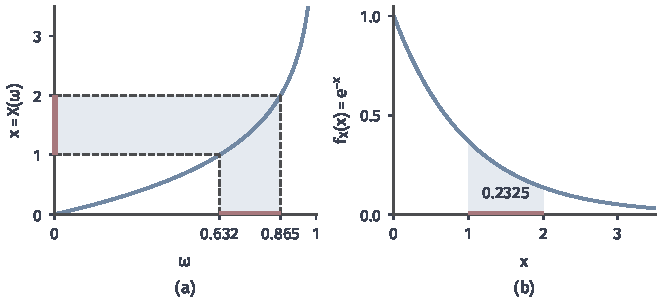
\includegraphics[width=112mm]{figures/07-probability/02-measure-theoretic-probability/matplotlib/pspace-pushforward-exp/figure.pdf}
  \caption{用原像计算推前分布。(a)蓝线是$x=X(\omega)=-\ln(1-\omega)$，纵轴上的红色线段是$B=(1,2]$，它的原像是横轴上的红色线段$(0.632,0.865]$，长度$\mathrm{e}^{-1}-\mathrm{e}^{-2}$；(b)取值空间上的分布，浅蓝面积是$P_X((1,2])\approx0.2325$。}
  \label{fig:pspace-pushforward-exp}
\end{BookInlineFigure}

对实值随机变量，分布函数$F_X(x)=P_X((-\infty,x])$就是式~\eqref{eq:pspace-cdf}对$P=P_X$的特例。由定理~\ref{thm:pspace-cdf-measure}，$F_X$确定了整个$P_X$：两个随机变量的分布函数相同，它们落在任何Borel集中的概率都相同。第~\ref{chap:random-variables}章只能从分布函数读出区间的概率，这一缺口现在补上了。

\paragraph{变换后的分布}
对随机对象再作可测变换$Y=g(X)$，$Y$的分布可以只用$X$的分布算出。对$B\in\mathcal{E}'$，$\{Y\in B\}=\{X\in g^{-1}(B)\}$，所以
\begin{equation}
  P_{g(X)}(B)=P_X\bigl(g^{-1}(B)\bigr).
  \label{eq:pspace-transform-law}
\end{equation}
质量先由$X$从$\Omega$搬到$E$，再由$g$从$E$搬到$E'$，两次搬运的结果与一次搬运$g\circ X$相同。

截断的等待时间是一个例子。对指数变量$X$取$Y=\min\{X,2\}$，即$g(x)=\min\{x,2\}$。单点$\{2\}$的原像是$[2,\infty)$，由式~\eqref{eq:pspace-transform-law}，
\[
  P_Y(\{2\})=P_X\bigl([2,\infty)\bigr)=\mathrm{e}^{-2}\approx0.1353,
\]
而$y<2$时$P_Y((-\infty,y])=P_X((-\infty,y])$。$X$在$[2,\infty)$上的质量全部被搬到点$2$上，所以$Y$的分布在$2$处有一个原子，这就是第~\ref{chap:random-variables}章在分布函数上看到的跳跃。第~\ref{chap:random-variable-transformations}章的各种换元公式，都是在具体的$g$下计算式~\eqref{eq:pspace-transform-law}；离散、连续和混合的情形使用的是同一条原像规则。

\paragraph{任何分布函数都可以实现}
定理~\ref{thm:pspace-cdf-measure}在实轴上造出了以$F$为分布函数的概率测度。能否在某个概率空间上造出一个随机变量，使它的分布函数恰好是$F$？最直接的办法是把$(\mathbb{R},\mathcal{B}(\mathbb{R}),P)$本身当作样本空间，令$X(x)=x$。下面给出另一种构造，它只用木棍上的一个均匀点，后面构造独立序列时会反复用到。

对满足定理~\ref{thm:pspace-cdf-measure}条件的$F$，定义
\begin{equation}
  Q(u)=\inf\{x\in\mathbb{R}:\ F(x)\geq u\},\qquad 0<u<1 .
  \label{eq:pspace-quantile}
\end{equation}
这就是第~\ref{chap:random-variables}章的分位数函数。$0<u<1$保证集合$\{x:F(x)\geq u\}$非空（因为$F\to1$）且有下界（因为$F\to0$），所以$Q(u)$是有限实数。

\begin{lemma}[分位数函数的基本关系]
\label{lem:pspace-quantile}
对$0<u<1$与$x\in\mathbb{R}$，
\begin{equation}
  Q(u)\leq x\iff u\leq F(x).
  \label{eq:pspace-quantile-galois}
\end{equation}
\end{lemma}

\begin{proof}
若$u\leq F(x)$，则$x$属于集合$\{y:F(y)\geq u\}$，下确界不超过它，即$Q(u)\leq x$。

反过来，先证下确界本身属于这个集合。取集合中的一列点$y_n\downarrow Q(u)$，每个都满足$F(y_n)\geq u$。由右连续性，
\[
  F\bigl(Q(u)\bigr)=\lim_{n\to\infty}F(y_n)\geq u .
\]
于是若$Q(u)\leq x$，由$F$单调不减得$F(x)\geq F(Q(u))\geq u$。
\end{proof}

\begin{theorem}[分位数变换]
\label{thm:pspace-quantile-transform}
设$F$满足定理~\ref{thm:pspace-cdf-measure}的条件，$Q$由式~\eqref{eq:pspace-quantile}定义。在$\Omega=[0,1)$、$\mathcal{F}=\mathcal{B}([0,1))$、$\mathbb{P}=\lambda$上，令$X(\omega)=Q(\omega)$（$\omega>0$），$X(0)=0$。则$X$是随机变量，且$F_X=F$。
\end{theorem}

\begin{proof}
对$x\in\mathbb{R}$，由式~\eqref{eq:pspace-quantile-galois}，
\[
  \{\omega\in(0,1):X(\omega)\leq x\}=\{\omega\in(0,1):\omega\leq F(x)\}=(0,F(x)]\cap(0,1).
\]
$\{X\leq x\}$是这个区间与可能的单点$\{0\}$之并，是Borel集，由判别~\eqref{eq:pspace-rv-criterion}，$X$是随机变量。单点概率为零，所以
\[
  \mathbb{P}(X\leq x)=\lambda\bigl((0,F(x)]\cap(0,1)\bigr)=F(x),
\]
最后一步在$F(x)=1$时也成立，因为$(0,1)$的长度是$1$。
\end{proof}

用等待时间$W$走一遍。分布函数在$t\geq0$时为$F_W(t)=0.3+0.7(1-\mathrm{e}^{-t})$，在$0$处从$0$跳到$0.3$。由式~\eqref{eq:pspace-quantile}，$u\leq0.3$时最小的满足$F_W(x)\geq u$的点是$0$；$u>0.3$时解方程$F_W(x)=u$。于是
\begin{equation}
  Q_W(u)=\begin{cases}0,&0<u\leq0.3,\\ \ln\dfrac{0.7}{1-u},&0.3<u<1.\end{cases}
  \label{eq:pspace-waiting-quantile}
\end{equation}
取两个均匀随机数$u=0.2$与$u=0.37$，得到
\[
  Q_W(0.2)=0,\qquad Q_W(0.37)=\ln\frac{0.7}{0.63}=\ln\frac{10}{9}\approx0.1054 .
\]
第一个落在跳跃的高度范围内，对应“不用等”；第二个对应等待约$0.105$个单位时间。图~\ref{fig:pspace-quantile-transform}显示，分布函数在$0$处的跳跃，变成了分位数函数在$(0,0.3]$上的平台：长度为$0.3$的一段均匀质量全部被送到点$0$。

\begin{BookInlineFigure}
  \centering
  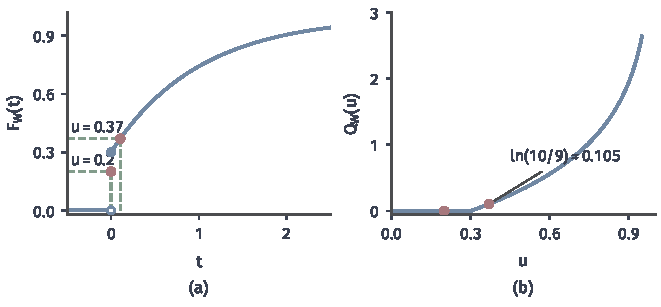
\includegraphics[width=112mm]{figures/07-probability/02-measure-theoretic-probability/matplotlib/pspace-quantile-transform/figure.pdf}
  \caption{用分位数变换从均匀随机数得到等待时间$W$。(a)蓝线是$F_W$；绿色虚线从高度$u$水平向右，碰到曲线（或跳跃的竖直段）后竖直向下，落点就是$Q_W(u)$；$u=0.2$落在跳跃内，得到$0$，$u=0.37$得到$\ln(10/9)$。(b)蓝线是$Q_W$，它在$(0,0.3]$上为$0$，红点是两个例子。}
  \label{fig:pspace-quantile-transform}
\end{BookInlineFigure}

定理~\ref{thm:pspace-quantile-transform}对Cantor分布同样适用，于是Cantor变量可以由一个均匀随机点得到。它也是从均匀随机数生成任意一维分布样本的基本方法，第~\ref{chap:sample-generation}章将讨论它的计算问题。

\paragraph{三种相等}
两个随机变量“相同”可以有三种不同强度的意思。设$X,Y$是同一概率空间上的随机变量。若对每个$\omega$都有$X(\omega)=Y(\omega)$，称它们处处相等；若$\mathbb{P}(X=Y)=1$，称它们几乎必然相等。第三种只比较分布，两个变量甚至可以定义在不同的概率空间上。

\begin{definition}[同分布]
\label{def:pspace-equal-in-law}
若随机对象$X$与$Y$取值于同一可测空间，且$P_X=P_Y$，则称$X$与$Y$同分布，记作
\begin{equation}
  X\overset{\mathrm{d}}{=}Y .
  \label{eq:pspace-equal-in-law}
\end{equation}
\end{definition}

三者依次减弱。处处相等时$\{X\neq Y\}=\varnothing$，所以处处相等蕴含几乎必然相等。若$X=Y$几乎必然成立，记$N=\{X\neq Y\}$，则对每个Borel集$B$，$\{X\in B\}$与$\{Y\in B\}$只在$N$中可能不同，它们的对称差包含于$N$，所以
\[
  \bigl\lvert P_X(B)-P_Y(B)\bigr\rvert\leq\mathbb{P}(N)=0,
\]
即$X\overset{\mathrm{d}}{=}Y$。

反方向都不成立。在木棍模型上取$U(\omega)=\omega$与$1-U$。对$u\in[0,1)$，
\[
  \mathbb{P}(1-U\leq u)=\mathbb{P}(U\geq1-u)=u,
\]
所以$1-U$也是均匀分布，$U\overset{\mathrm{d}}{=}1-U$。可是$U=1-U$只在$\omega=1/2$成立，$\mathbb{P}(U=1-U)=0$：两个同分布的变量几乎处处不相等，见图~\ref{fig:pspace-three-equalities}(a)。另一方面，把$U$在可数个点上改成$0$得到$U'$，例如在$\omega=k/8$（$k=1,\dots,7$）处，则$U'\neq U$只在一个零概率事件上发生，$U'=U$几乎必然成立，却不处处成立，见图~\ref{fig:pspace-three-equalities}(b)。

\begin{BookInlineFigure}
  \centering
  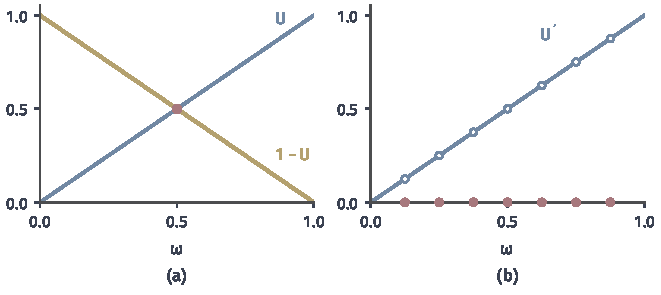
\includegraphics[width=112mm]{figures/07-probability/02-measure-theoretic-probability/matplotlib/pspace-three-equalities/figure.pdf}
  \caption{三种相等的区别，横轴是样本点$\omega\in[0,1)$。(a)蓝线$U(\omega)=\omega$与黄线$1-U$只在红点$\omega=1/2$处相等，二者却同为均匀分布；(b)$U'$在$\omega=k/8$处被改为$0$（红点），空心点是原来的值，其余位置与$U$相同，二者几乎必然相等。}
  \label{fig:pspace-three-equalities}
\end{BookInlineFigure}

这三种相等在实践中各有用处。一切只依赖分布的量，例如$\mathbb{P}(X>2)$、分位数以及第~\ref{sec:pspace-expectation}节将统一定义的期望，对同分布的变量都相同。几乎必然相等的变量还能在同一个样本点上互相替换，这在讨论多个变量的组合时是必需的。处处相等很少需要，因为零概率事件上的差别不影响任何概率。

\paragraph{边缘分布不能确定配对}
同分布的变量不能随意替换进组合中。仍取$X=U$与$X'=1-U$，二者同分布；再取$Y=U$，则
\[
  X+Y=2U,\qquad X'+Y=1 .
\]
前者均匀分布在$[0,2)$上，后者恒等于$1$。原因是$X+Y$的分布不只依赖$X$和$Y$各自的分布，还依赖它们在同一个样本点上怎样配对。

配对由联合分布描述。$(X,Y)$是取值于$\mathbb{R}^{2}$的随机向量，它的分布$P_{(X,Y)}$称为联合分布；$X$的分布是它在坐标投影$\pi_1(x,y)=x$下的推前，
\[
  P_X(B)=\mathbb{P}\bigl((X,Y)\in B\times\mathbb{R}\bigr)=P_{(X,Y)}\bigl(\pi_1^{-1}(B)\bigr).
\]
差$X-Y$是映射$(x,y)\mapsto x-y$下的推前，所以它的分布由联合分布确定，却不能由两个边缘分布确定。

下面三种配对的边缘都是$[0,1)$上的均匀分布：$(U,U)$、$(U,1-U)$，以及$(U,V)$，其中$V$是与$U$独立的另一个均匀变量（第~\ref{sec:pspace-independence}节在同一个概率空间上构造它）。记$D=X-Y$，三种配对下：
\begin{enumerate}
  \item $(U,U)$：$D\equiv0$，质量全部集中在原点；
  \item $(U,1-U)$：$D=2U-1$，均匀分布在$(-1,1)$上，密度为$1/2$；
  \item $(U,V)$：$D$的密度是$1-\lvert z\rvert$（$\lvert z\rvert<1$），即第~\ref{chap:random-variable-transformations}章算过的三角形密度。
\end{enumerate}
差的大小随配对变化很大。以$\mathbb{P}(\lvert D\rvert\leq0.1)$为例，三种配对依次是
\[
  1,\qquad \frac{0.2}{2}=0.1,\qquad 1-0.9^{2}=0.19 .
\]
第三个数是三角形密度在$[-0.1,0.1]$上的积分，等于$1$减去两侧两个直角三角形的面积$2\times\frac12\times0.9^{2}$。$D$的方差依次为$0$、$1/3$和$1/6$。

\begin{BookInlineFigure}
  \centering
  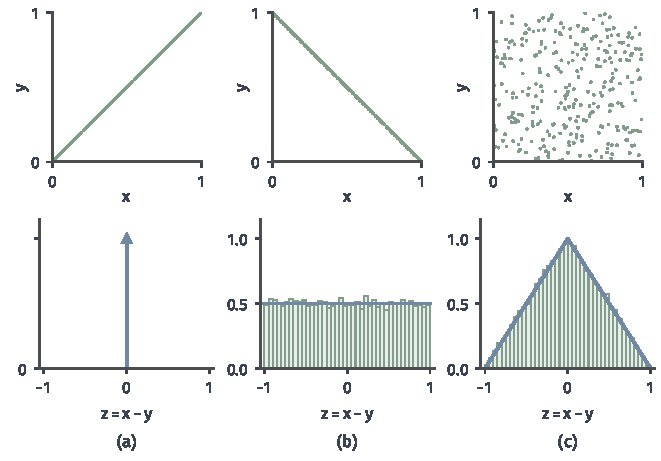
\includegraphics[width=112mm]{figures/07-probability/02-measure-theoretic-probability/matplotlib/pspace-couplings/figure.pdf}
  \caption{三种边缘相同的配对。上行是$300$对模拟样本（种子$9$）的散点：(a)$(U,U)$落在对角线上，(b)$(U,1-U)$落在反对角线上，(c)独立的$(U,V)$铺满正方形。下行是$D=X-Y$的分布：(a)全部质量在$0$（箭头表示单点质量$1$），(b)(c)中浅绿直方图来自$20000$对模拟样本，蓝线分别是均匀密度$1/2$与三角形密度$1-\lvert z\rvert$。}
  \label{fig:pspace-couplings}
\end{BookInlineFigure}

图~\ref{fig:pspace-couplings}的上行显示，三种配对的质量在平面上的位置完全不同，但向两条坐标轴的投影都是均匀分布。把同一组边缘分布配成联合分布的方式称为耦合，第~\ref{chap:optimal-transport}章研究怎样选择耦合使搬运代价最小。本章需要记住的是：随机变量本身、它的分布和多个变量的联合分布是三个不同层次的对象，从后者可以推出前者，反之不能。

\section{独立构造}
\label{sec:pspace-independence}

第~\ref{chap:random-vectors}章用乘法公式定义了随机变量的独立：对区间、概率表或密度，联合概率等于边缘概率之积。那里留下两个问题。其一，乘法公式只在区间或矩形上验证过，能否推出它对一切Borel集都成立？其二，第~\ref{chap:random-variables}章构造Cantor变量时，直接使用了“无穷多次独立抛硬币”，这样的模型是否存在？本节先回答第一个问题，然后用乘积测度和二进制数字回答第二个问题。

\paragraph{信息族的独立}
独立的直观含义是：知道一个对象的取值，不改变另一个对象落在各处的概率。用上一节的语言，一个随机对象提供的信息是它生成的$\sigma$代数，所以最自然的定义是在$\sigma$代数之间写乘法公式。

\begin{definition}[独立]
\label{def:pspace-independence}
设$\mathcal{G}_1,\dots,\mathcal{G}_n$是$\mathcal{F}$的子$\sigma$代数。若对任意$A_1\in\mathcal{G}_1,\dots,A_n\in\mathcal{G}_n$都有
\begin{equation}
  \mathbb{P}(A_1\cap\cdots\cap A_n)=\mathbb{P}(A_1)\cdots\mathbb{P}(A_n),
  \label{eq:pspace-independence}
\end{equation}
则称它们相互独立。任意一族子$\sigma$代数$\{\mathcal{G}_i\}_{i\in I}$称为相互独立，若其中每个有限子族都相互独立。随机对象$\{X_i\}_{i\in I}$相互独立，是指$\{\sigma(X_i)\}_{i\in I}$相互独立。
\end{definition}

对随机对象，式~\eqref{eq:pspace-independence}就是对一切可测集$B_i$，
\[
  \mathbb{P}(X_1\in B_1,\dots,X_n\in B_n)=\mathbb{P}(X_1\in B_1)\cdots\mathbb{P}(X_n\in B_n).
\]
对事件，$A_1,\dots,A_n$独立是指$\sigma(\{A_1\}),\dots,\sigma(\{A_n\})$独立。每个$\sigma(\{A_i\})$都含有$\Omega$，在式~\eqref{eq:pspace-independence}中把一部分$A_i$换成$\Omega$，就得到对子族的乘法公式；换成$A_i^{\mathrm{c}}$，就得到补事件的乘法公式。所以这与第~\ref{chap:classical-probability}章“每个子族都满足乘法公式”的定义一致。

\paragraph{只需在生成族上检验}
定义要求对$\sigma$代数中的\emph{所有}事件检验乘法公式，而$\mathcal{B}(\mathbb{R})$中的集合无法逐一列出。下面的引理说明，在一个对交封闭的生成族上检验就够了。

\begin{lemma}[独立性的$\pi$系统判据]
\label{lem:pspace-pi-independence}
设$\mathcal{C}_1,\dots,\mathcal{C}_n\subseteq\mathcal{F}$都是$\pi$系统，且$\Omega\in\mathcal{C}_i$。若对任意$C_1\in\mathcal{C}_1,\dots,C_n\in\mathcal{C}_n$都有
\begin{equation}
  \mathbb{P}(C_1\cap\cdots\cap C_n)=\mathbb{P}(C_1)\cdots\mathbb{P}(C_n),
  \label{eq:pspace-pi-independence}
\end{equation}
则$\sigma(\mathcal{C}_1),\dots,\sigma(\mathcal{C}_n)$相互独立。
\end{lemma}

\begin{proof}
固定$C_2\in\mathcal{C}_2,\dots,C_n\in\mathcal{C}_n$，记$R=C_2\cap\cdots\cap C_n$，$r=\mathbb{P}(C_2)\cdots\mathbb{P}(C_n)$。令
\[
  \mathcal{D}=\bigl\{A\in\mathcal{F}:\ \mathbb{P}(A\cap R)=\mathbb{P}(A)\,r\bigr\}.
\]
由假设$\mathcal{C}_1\subseteq\mathcal{D}$。下面验证$\mathcal{D}$是卷四意义下的$\lambda$系统。

第一，$\Omega\in\mathcal{C}_1\subseteq\mathcal{D}$，这一步说明了为什么要求$\Omega\in\mathcal{C}_i$：取$A=\Omega$得到$\mathbb{P}(R)=r$。第二，若$A\in\mathcal{D}$，则
\[
  \mathbb{P}(A^{\mathrm{c}}\cap R)=\mathbb{P}(R)-\mathbb{P}(A\cap R)=r-\mathbb{P}(A)\,r=\mathbb{P}(A^{\mathrm{c}})\,r,
\]
所以$A^{\mathrm{c}}\in\mathcal{D}$。第三，若$A_1,A_2,\dots\in\mathcal{D}$两两不交，由可数可加性，
\[
  \mathbb{P}\Bigl(\bigcup_kA_k\cap R\Bigr)=\sum_k\mathbb{P}(A_k\cap R)=\sum_k\mathbb{P}(A_k)\,r=\mathbb{P}\Bigl(\bigcup_kA_k\Bigr)r .
\]

由$\pi$--$\lambda$定理，$\sigma(\mathcal{C}_1)\subseteq\mathcal{D}$。这说明式~\eqref{eq:pspace-pi-independence}在把$\mathcal{C}_1$换成$\sigma(\mathcal{C}_1)$后仍然成立，而$\sigma(\mathcal{C}_1)$也是含$\Omega$的$\pi$系统。对第二个指标重复同样的论证，把$\mathcal{C}_2$换成$\sigma(\mathcal{C}_2)$；依次做$n$次，就得到$\sigma(\mathcal{C}_1),\dots,\sigma(\mathcal{C}_n)$满足式~\eqref{eq:pspace-independence}。
\end{proof}

最重要的应用是用分布函数判断独立，它补上第~\ref{chap:random-vectors}章留下的一步。

\begin{theorem}[独立的分布函数判据]
\label{thm:pspace-cdf-independence}
实值随机变量$X_1,\dots,X_n$相互独立，当且仅当对一切$x_1,\dots,x_n\in\mathbb{R}$，
\begin{equation}
  \mathbb{P}(X_1\leq x_1,\dots,X_n\leq x_n)=F_{X_1}(x_1)\cdots F_{X_n}(x_n).
  \label{eq:pspace-cdf-independence}
\end{equation}
\end{theorem}

\begin{proof}
必要性是定义取$B_i=(-\infty,x_i]$的特例。对充分性，令
\[
  \mathcal{C}_i=\bigl\{\{X_i\leq x\}:x\in\mathbb{R}\bigr\}\cup\{\Omega\}.
\]
它对交封闭，因为两个半直线事件之交仍是半直线事件，顶点取较小者（图~\ref{fig:pspace-pi-system}画出了二维的情形）。

式~\eqref{eq:pspace-pi-independence}在所有$C_i$都取半直线事件时就是式~\eqref{eq:pspace-cdf-independence}。若某些$C_i=\Omega$，对相应的$x_i\to+\infty$取极限：左边的事件递增到去掉这些坐标后的事件，由连续性，两边分别收敛到去掉这些因子后的形式，乘法公式仍成立。

最后，$\sigma(\mathcal{C}_i)=\sigma(X_i)$。一方面$\mathcal{C}_i\subseteq\sigma(X_i)$。另一方面，使$X_i^{-1}(B)\in\sigma(\mathcal{C}_i)$的Borel集$B$构成$\sigma$代数，它含有全部半直线，因而含有$\mathcal{B}(\mathbb{R})$。由引理~\ref{lem:pspace-pi-independence}，$\sigma(X_1),\dots,\sigma(X_n)$相互独立。
\end{proof}

\begin{BookInlineFigure}
  \centering
  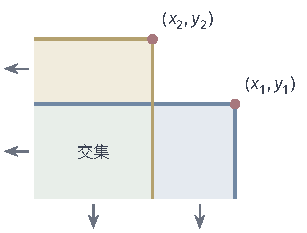
\includegraphics[width=52mm]{figures/07-probability/02-measure-theoretic-probability/tikz/pspace-pi-system/figure.pdf}
  \caption{左下象限构成$\pi$系统。以$(x_1,y_1)$为顶点的象限（浅蓝，蓝色边界）与以$(x_2,y_2)$为顶点的象限（浅黄，黄色边界）都向左、向下无限延伸，它们的交集（浅绿）仍是左下象限，顶点为$(\min\{x_1,x_2\},\min\{y_1,y_2\})$。}
  \label{fig:pspace-pi-system}
\end{BookInlineFigure}

\paragraph{分组保持独立}
第~\ref{chap:random-vectors}章还使用过一个事实：相互独立的变量分成互不相交的几组，各组的函数仍相互独立，例如$X_1+X_2$与$X_3^{2}$独立。现在可以对一般的可测函数证明它。

\begin{theorem}[分组定理]
\label{thm:pspace-grouping}
设$\{\mathcal{G}_i\}_{i\in I}$相互独立，$I_1,I_2,\dots$是$I$的两两不交的子集。令$\mathcal{H}_k$为由$\bigcup_{i\in I_k}\mathcal{G}_i$生成的$\sigma$代数。则$\mathcal{H}_1,\mathcal{H}_2,\dots$相互独立。
\end{theorem}

\begin{proof}
只需证明任意有限个$\mathcal{H}_1,\dots,\mathcal{H}_m$相互独立。令$\mathcal{C}_k$为形如$A_{i_1}\cap\cdots\cap A_{i_r}$的集合全体，其中$i_1,\dots,i_r$是$I_k$中有限个不同的指标，$A_{i_j}\in\mathcal{G}_{i_j}$。$\mathcal{C}_k$对交封闭，含有$\Omega$，且生成$\mathcal{H}_k$。

取$C_k\in\mathcal{C}_k$，$k=1,\dots,m$。不同组的指标互不相同，$C_1\cap\cdots\cap C_m$是来自有限个不同$\mathcal{G}_i$的事件之交。由$\{\mathcal{G}_i\}$的独立性，它的概率等于所有这些事件的概率之积；把乘积按组归并，又等于$\mathbb{P}(C_1)\cdots\mathbb{P}(C_m)$。由引理~\ref{lem:pspace-pi-independence}，$\mathcal{H}_1,\dots,\mathcal{H}_m$相互独立。
\end{proof}

若$X_1,X_2,X_3$相互独立，取$I_1=\{1,2\}$，$I_2=\{3\}$，则$\sigma(X_1,X_2)$与$\sigma(X_3)$独立。这里用到$\sigma(X_1,X_2)$就是由$\sigma(X_1)\cup\sigma(X_2)$生成的$\sigma$代数，因为$\mathcal{B}(\mathbb{R}^{2})$由矩形$B_1\times B_2$生成，而矩形的原像是
\[
  \{(X_1,X_2)\in B_1\times B_2\}=\{X_1\in B_1\}\cap\{X_2\in B_2\}.
\]
对任意Borel函数$g,h$，由上一节“函数只会减少信息”，$\sigma(g(X_1,X_2))\subseteq\sigma(X_1,X_2)$，$\sigma(h(X_3))\subseteq\sigma(X_3)$，所以$g(X_1,X_2)$与$h(X_3)$独立。$g$、$h$不必连续，也不必使原像是区间。

\paragraph{乘积测度给出独立对}
现在转向构造。给定两个概率空间$(E_1,\mathcal{E}_1,P_1)$与$(E_2,\mathcal{E}_2,P_2)$，要造一对独立的随机对象，分布分别是$P_1$和$P_2$。卷四的乘积测度正好做这件事：在$E_1\times E_2$上，乘积$\sigma$代数$\mathcal{E}_1\otimes\mathcal{E}_2$由可测矩形$A\times B$生成，其上存在唯一的概率测度$P_1\otimes P_2$，使
\begin{equation}
  (P_1\otimes P_2)(A\times B)=P_1(A)\,P_2(B),\qquad A\in\mathcal{E}_1,\ B\in\mathcal{E}_2 .
  \label{eq:pspace-product-measure}
\end{equation}
取$\Omega=E_1\times E_2$与$\mathbb{P}=P_1\otimes P_2$，令$X$、$Y$分别取$\omega=(\omega_1,\omega_2)$的第一、第二个坐标。这时
\[
  \{X\in A\}\cap\{Y\in B\}=A\times B,
\]
式~\eqref{eq:pspace-product-measure}说的正是$X$与$Y$独立，且$P_X=P_1$，$P_Y=P_2$。

反过来，独立性也可以完全用联合分布刻画。

\begin{theorem}[独立与乘积分布]
\label{thm:pspace-independence-product}
设$X,Y$分别取值于$(E_1,\mathcal{E}_1)$与$(E_2,\mathcal{E}_2)$。则$X$与$Y$独立，当且仅当
\begin{equation}
  P_{(X,Y)}=P_X\otimes P_Y .
  \label{eq:pspace-independence-product}
\end{equation}
\end{theorem}

\begin{proof}
若式~\eqref{eq:pspace-independence-product}成立，在矩形上取值就得到$\mathbb{P}(X\in A,Y\in B)=P_X(A)P_Y(B)$，即独立。反过来，若$X,Y$独立，则$P_{(X,Y)}$与$P_X\otimes P_Y$在全部可测矩形上取值相同。可测矩形对交封闭，因为
\[
  (A\times B)\cap(A'\times B')=(A\cap A')\times(B\cap B'),
\]
并且它们生成$\mathcal{E}_1\otimes\mathcal{E}_2$。两个概率测度在生成的$\pi$系统上一致，就处处一致。
\end{proof}

这个定理把“独立”从样本空间上的乘法公式，变成了取值空间上的一句话：联合分布是边缘分布的乘积。有密度时可以进一步写成密度的乘积。设$X,Y$分别有密度$f_X,f_Y$。由Tonelli定理，对矩形，
\[
  (P_X\otimes P_Y)(A\times B)=\int_Af_X\,\mathrm{d}x\int_Bf_Y\,\mathrm{d}y=\iint_{A\times B}f_X(x)f_Y(y)\,\mathrm{d}x\,\mathrm{d}y,
\]
再用$\pi$系统论证推广到一切Borel集，所以$f_X(x)f_Y(y)$是$P_X\otimes P_Y$的密度。于是：$X$与$Y$独立，当且仅当$f_X(x)f_Y(y)$是$(X,Y)$的一个联合密度。若$(X,Y)$另有联合密度$f$，同一个测度的两个密度只能在Lebesgue测度为零的集合上不同，可参考\BookChapterRef{chap:measure-densities}{卷四第8章“测度的密度”}；所以独立等价于$f=f_Xf_Y$几乎处处成立。这正是第~\ref{chap:random-vectors}章提到的情形：把联合密度在一条直线上改掉，它仍是联合密度，独立性不受影响。

\paragraph{一个独立对的计算}
设$X\sim\operatorname{Unif}(0,1)$，$Y\sim\operatorname{Exp}(1)$，二者独立，即$(X,Y)$的分布是$\operatorname{Unif}(0,1)\otimes\operatorname{Exp}(1)$。矩形事件直接相乘：
\[
  \mathbb{P}\bigl(X\leq\tfrac12,\ Y>1\bigr)=\tfrac12\cdot\mathrm{e}^{-1}\approx0.1839 .
\]
非矩形事件要对乘积测度积分。事件$\{Y>X\}$是正方形上方、对角线以上的区域。按$x$切片，每条竖直切片$\{y>x\}$在$Y$的分布下的质量是$\mathrm{e}^{-x}$，再对$x$在均匀分布下积分：
\[
  \mathbb{P}(Y>X)=\int_0^1\mathbb{P}(Y>x)\,\mathrm{d}x=\int_0^1\mathrm{e}^{-x}\,\mathrm{d}x=1-\mathrm{e}^{-1}\approx0.6321 .
\]
图~\ref{fig:pspace-product-measure}画出了这两个事件。第二步按切片积分的依据是Tonelli定理：被积函数是区域的示性函数，非负，可以先对$y$积分再对$x$积分。

\begin{BookInlineFigure}
  \centering
  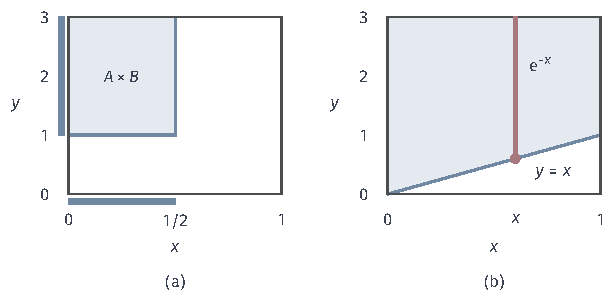
\includegraphics[width=104mm]{figures/07-probability/02-measure-theoretic-probability/tikz/pspace-product-measure/figure.pdf}
  \caption{$\operatorname{Unif}(0,1)\otimes\operatorname{Exp}(1)$上的两个事件，纵轴只画到$y=3$，区域向上延伸。(a)矩形$A\times B$，$A=[0,\tfrac12]$，$B=(1,\infty)$（坐标轴旁的粗线段），概率是两段边缘概率之积；(b)区域$\{y>x\}$，红色竖线是$x$处的切片，它在$Y$的分布下的质量是$\mathrm{e}^{-x}$。}
  \label{fig:pspace-product-measure}
\end{BookInlineFigure}

\paragraph{无穷多次抛硬币}
有限个独立对象由有限次乘积得到，可数个则需要无穷乘积。对实值的情形，木棍上的一个均匀点已经足够。仍取$\Omega=[0,1)$、长度测度，以及上一节的二进制数字$D_k(\omega)$。

\begin{theorem}[二进制数字独立]
\label{thm:pspace-binary-digits}
在$([0,1),\mathcal{B}([0,1)),\lambda)$上，$D_1,D_2,\dots$相互独立，且都服从$\operatorname{Bern}(1/2)$。
\end{theorem}

\begin{proof}
固定$n$与$d_1,\dots,d_n\in\{0,1\}$，令$a=\sum_{k=1}^{n}d_k2^{-k}$。按$D_k$的定义，$\omega$的前$n$位数字依次是$d_1,\dots,d_n$，当且仅当$\lfloor2^{n}\omega\rfloor=2^{n}a$，即
\[
  \{D_1=d_1,\dots,D_n=d_n\}=\bigl[a,\ a+2^{-n}\bigr).
\]
这个区间的长度是$2^{-n}$，所以
\[
  \mathbb{P}(D_1=d_1,\dots,D_n=d_n)=2^{-n}.
\]

对单个数字，把前$n$位中其余$n-1$位的所有取值加起来，得$\mathbb{P}(D_k=d)=2^{n-1}\cdot2^{-n}=1/2$。于是对前$n$个数字，联合概率等于各自概率之积。任意有限个数字都包含在某个前$n$个之中，对不出现的数字求和即可，所以任意有限子族满足乘法公式。数字只取两个值，$\sigma(D_k)$由$\{D_k=1\}$生成，乘法公式对$\sigma(D_k)$中的四个事件都成立。
\end{proof}

图~\ref{fig:pspace-binary-digits}画出了前三位数字。事件$\{D_1=1,D_3=0\}$由两段长$1/8$的区间组成，总长度$1/4=\frac12\cdot\frac12$，与乘法公式一致。

\begin{BookInlineFigure}
  \centering
  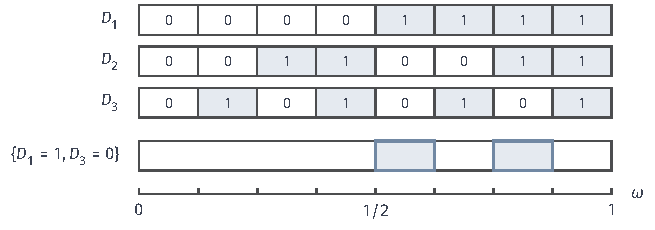
\includegraphics[width=111mm]{figures/07-probability/02-measure-theoretic-probability/tikz/pspace-binary-digits/figure.pdf}
  \caption{$[0,1)$上的二进制数字。前三行中，每个长$1/8$的格子里写着其中各点的第$k$位数字，浅蓝格子取值为$1$。最下一行是事件$\{D_1=1,D_3=0\}=[\tfrac12,\tfrac58)\cup[\tfrac34,\tfrac78)$，长度$\tfrac14$。}
  \label{fig:pspace-binary-digits}
\end{BookInlineFigure}

于是“无穷多次独立抛公平硬币”有了一个具体模型：样本点是木棍上的一个点，第$k$次的结果是它的第$k$位二进制数字。第~\ref{chap:random-variables}章的Cantor变量$\sum_k2D_k/3^{k}$就定义在这个空间上。“首次出现正面的次数”$T=\min\{k:D_k=1\}$也是如此，事件“永远不出现正面”是$\{T=\infty\}=\{0\}$：它非空，概率却为零，是第~\ref{sec:pspace-null-events}节所说的零概率而非不可能事件。

\paragraph{可数个独立的任意分布}
一个均匀点的数字可以拆成可数多组，每组再拼成一个均匀点。正整数$n$可以唯一地写成$n=2^{k-1}(2j-1)$，其中$k,j\geq1$：$k-1$是$n$中因子$2$的个数，$2j-1$是剩下的奇数部分。于是位置集合
\[
  I_k=\{2^{k-1}(2j-1):\ j=1,2,\dots\},\qquad k=1,2,\dots
\]
两两不交，并且覆盖全部正整数。令
\begin{equation}
  U_k=\sum_{j=1}^{\infty}D_{2^{k-1}(2j-1)}\,2^{-j},
  \label{eq:pspace-digit-split}
\end{equation}
即用第$k$组数字依次作为$U_k$的二进制数字（图~\ref{fig:pspace-digit-interleave}）。

\begin{BookInlineFigure}
  \centering
  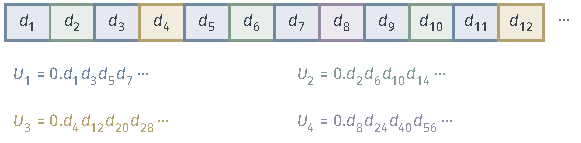
\includegraphics[width=98mm]{figures/07-probability/02-measure-theoretic-probability/tikz/pspace-digit-interleave/figure.pdf}
  \caption{把一个均匀点的二进制数字$d_1d_2d_3\cdots$分成互不相交的组。第$k$组由位置$2^{k-1}(2j-1)$组成，颜色相同的格子属于同一组：奇数位置给$U_1$（蓝），$2,6,10,\dots$给$U_2$（绿），$4,12,20,\dots$给$U_3$（黄），$8,24,\dots$给$U_4$（紫）。}
  \label{fig:pspace-digit-interleave}
\end{BookInlineFigure}

\begin{theorem}[独立序列的存在]
\label{thm:pspace-independent-sequence}
设$F_1,F_2,\dots$是一列满足定理~\ref{thm:pspace-cdf-measure}条件的函数。则在$([0,1),\mathcal{B}([0,1)),\lambda)$上存在相互独立的随机变量$X_1,X_2,\dots$，使$F_{X_k}=F_k$对每个$k$成立。
\end{theorem}

\begin{proof}
分三步。第一步说明$U_1,U_2,\dots$相互独立。$U_k$是第$k$组数字的部分和之极限，可测函数列的极限可测，所以$U_k$关于$\mathcal{H}_k=\sigma(D_n:n\in I_k)$可测，$\sigma(U_k)\subseteq\mathcal{H}_k$。各组位置互不相交，由定理~\ref{thm:pspace-binary-digits}与分组定理~\ref{thm:pspace-grouping}，$\mathcal{H}_1,\mathcal{H}_2,\dots$相互独立，于是$U_1,U_2,\dots$相互独立。

第二步说明每个$U_k$都是均匀分布。$U_k$的数字序列与$(D_1,D_2,\dots)$同样是独立的公平比特。对二进分点区间$J=[b2^{-m},(b+1)2^{-m})$，$U_k\in J$意味着$U_k$的前$m$位数字是$b$的二进制表示，除非$U_k$的数字从某一位起全为$1$。后一情形的概率为零：对固定的起始位置，“此后$r$位全为$1$”的概率是$2^{-r}$，令$r\to\infty$得零，再对可数个起始位置取并。于是
\[
  \mathbb{P}(U_k\in J)=2^{-m}=\lambda(J).
\]
二进分点区间与空集一起构成$\pi$系统，生成$\mathcal{B}([0,1))$，并且$\mathbb{P}(U_k\in[0,1))=1$，所以$U_k$的分布就是长度测度。

第三步作分位数变换。令$Q_k$为$F_k$的分位数函数，$U_k\in(0,1)$时令$X_k=Q_k(U_k)$，否则令$X_k=0$。$U_k$均匀分布，由定理~\ref{thm:pspace-quantile-transform}的证明，$F_{X_k}=F_k$。每个$X_k$是$U_k$的函数，由分组定理，$X_1,X_2,\dots$相互独立。
\end{proof}

第一部分及后续各章常说“取独立同分布的$X_1,X_2,\dots$”，这个定理保证了这样的序列确实存在，而且可以放在同一个概率空间上。取值于$\mathbb{R}^{d}$时，把每个$U_k$的数字再拆成$d$组，就得到$d$个独立坐标。对任意一列概率空间$(E_k,\mathcal{E}_k,P_k)$，可数乘积$\bigotimes_kP_k$在由“只限制有限个坐标”的柱集生成的$\sigma$代数上也存在且唯一，这一般性结论需要测度延拓的进一步论证，篇幅较长，读者可查阅~\scite{math-kallenberg2021probability}。本卷用到的独立序列都是实值或向量值的，上面的构造已经够用。

指标不可数时情况不同。连续时间的随机过程$\{X_t\}_{t\geq0}$也可以按有限个时刻的联合分布在乘积空间上构造，但“路径连续”这样的性质涉及不可数个时刻，不是由有限个坐标决定的事件，第~\ref{sec:pspace-null-events}节的尖峰例子已经显示了这类困难。处理它需要选择合适的版本并证明路径的正则性，可参考\BookChapterRef{chap:stochastic-processes-and-information}{卷九第2章“随机过程与随时间增长的信息”}。

\section{期望的积分表示}
\label{sec:pspace-expectation}

第~\ref{chap:random-variable-moments}章把期望定义为概率表上的加权和或密度的积分，等待时间$W$只能把两部分拆开计算，Cantor变量的期望则无从下手。另外几个结论也留了下来：两个任意随机变量之和的期望、求和与取极限的交换、用密度直接计算$\mathbb{E}[g(X)]$的公式。这些都归结为同一件事：期望是随机变量对概率测度的积分。

\paragraph{非负随机变量}
最简单的随机变量只取有限个值。设$A_1,\dots,A_m$是$\Omega$的一个划分，各块都是事件，$a_i\geq0$，
\[
  X=\sum_{i=1}^{m}a_i\mathbf{1}_{A_i}.
\]
这样的$X$称为简单随机变量，它在每一块上取常数值。它的期望只能是按块加权：
\[
  \mathbb{E}[X]=\sum_{i=1}^{m}a_i\,\mathbb{P}(A_i),
\]
这与第~\ref{chap:random-variable-moments}章对有限取值变量的定义一致。一般的非负随机变量用从下方逼近它的简单随机变量来定义，这就是卷四对非负可测函数的积分。

\begin{definition}[非负随机变量的期望]
\label{def:pspace-expectation-nonnegative}
设$X\geq0$是随机变量。称
\begin{equation}
  \mathbb{E}[X]=\int_{\Omega}X\,\mathrm{d}\mathbb{P}=\sup\bigl\{\mathbb{E}[\varphi]:\ \varphi\text{ 是简单随机变量},\ 0\leq\varphi\leq X\bigr\}
  \label{eq:pspace-expectation-nonnegative}
\end{equation}
为$X$的期望，它的值属于$[0,+\infty]$。
\end{definition}

上确界并不需要逐个比较。卷四给出了一列标准的逼近：
\begin{equation}
  \varphi_n=\min\Bigl\{n,\ \frac{\lfloor2^{n}X\rfloor}{2^{n}}\Bigr\},\qquad n=1,2,\dots .
  \label{eq:pspace-simple-approx}
\end{equation}
$\varphi_n$把$X$的取值向下取整到$2^{-n}$的整数倍，并在$n$处截断，它只取有限个值，且$\varphi_n\uparrow X$。由单调收敛定理，$\mathbb{E}[\varphi_n]\uparrow\mathbb{E}[X]$。

这个逼近与黎曼积分的思路不同。黎曼积分切分的是定义域，在$\Omega$上切小块；这里切分的是取值，把$X$的值分成宽$2^{-n}$的层，每层的值乘以落在这层的概率再相加。$\Omega$可以是任何集合，没有“小块”可言，按取值分层却总能进行，所需的只是每层$\{k2^{-n}\leq X<(k+1)2^{-n}\}$是事件，也就是$X$的可测性。

在木棍模型上看$X(\omega)=-\ln(1-\omega)$，它服从$\operatorname{Exp}(1)$。$n=1$时$\varphi_1$取三个值，
\[
  \varphi_1=\begin{cases}0,&X<\tfrac12,\\ \tfrac12,&\tfrac12\leq X<1,\\ 1,&X\geq1,\end{cases}
\]
各层的概率由指数分布的尾概率算出，于是
\[
  \mathbb{E}[\varphi_1]=\tfrac12\bigl(\mathrm{e}^{-1/2}-\mathrm{e}^{-1}\bigr)+1\cdot\mathrm{e}^{-1}\approx0.1193+0.3679=0.4872 .
\]
继续加细，前几项依次为
\[
  \mathbb{E}[\varphi_1]\approx0.4872,\quad \mathbb{E}[\varphi_2]\approx0.7611,\quad \mathbb{E}[\varphi_3]\approx0.8921,\quad \mathbb{E}[\varphi_4]\approx0.9513,
\]
它们递增地趋于$\mathbb{E}[X]=1$（图~\ref{fig:pspace-simple-approx}）。

\begin{BookInlineFigure}
  \centering
  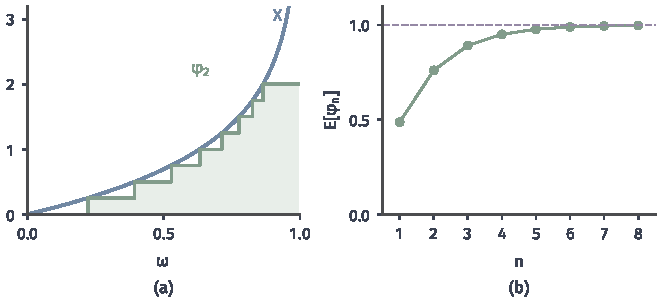
\includegraphics[width=112mm]{figures/07-probability/02-measure-theoretic-probability/matplotlib/pspace-simple-approx/figure.pdf}
  \caption{用简单随机变量逼近期望。(a)蓝线是$X(\omega)=-\ln(1-\omega)$，绿色阶梯是$\varphi_2$：取值向下取整到$1/4$的倍数并在$2$处截断，浅绿面积是$\mathbb{E}[\varphi_2]$；(b)绿点是$\mathbb{E}[\varphi_n]$，由式~\eqref{eq:pspace-simple-approx}按层精确算出，递增地趋于紫色虚线$\mathbb{E}[X]=1$。}
  \label{fig:pspace-simple-approx}
\end{BookInlineFigure}

\paragraph{有符号随机变量}
一般的随机变量拆成正部与负部，$X=X^{+}-X^{-}$，其中$X^{+}=\max\{X,0\}$，$X^{-}=\max\{-X,0\}$，两者都非负。

\begin{definition}[期望与可积]
\label{def:pspace-expectation}
设$X$是随机变量。若$\mathbb{E}[X^{+}]$与$\mathbb{E}[X^{-}]$至少有一个有限，定义
\begin{equation}
  \mathbb{E}[X]=\mathbb{E}[X^{+}]-\mathbb{E}[X^{-}].
  \label{eq:pspace-expectation}
\end{equation}
若$\mathbb{E}[X^{+}]$与$\mathbb{E}[X^{-}]$都有限，即$\mathbb{E}[\lvert X\rvert]<\infty$，称$X$可积。
\end{definition}

两部分都为无穷时期望没有定义，这正是第~\ref{chap:common-distributions}章对Cauchy分布的结论。可积的随机变量构成一个向量空间，期望是它上面的线性函数。

\begin{theorem}[期望的基本性质]
\label{thm:pspace-expectation-properties}
设$X,Y$是可积随机变量，$a,b\in\mathbb{R}$。
\begin{enumerate}
  \item 线性：$aX+bY$可积，且
  \begin{equation}
    \mathbb{E}[aX+bY]=a\,\mathbb{E}[X]+b\,\mathbb{E}[Y];
    \label{eq:pspace-linearity}
  \end{equation}
  \item 保序：若$X\leq Y$几乎必然成立，则$\mathbb{E}[X]\leq\mathbb{E}[Y]$；
  \item 绝对值估计：$\lvert\mathbb{E}[X]\rvert$不超过$\mathbb{E}[\lvert X\rvert]$；
  \item 若$X=Y$几乎必然成立，则$\mathbb{E}[X]=\mathbb{E}[Y]$；
  \item 若$X\geq0$且$\mathbb{E}[X]=0$，则$X=0$几乎必然成立。
\end{enumerate}
\end{theorem}

\begin{proof}
前四条是卷四积分的线性、单调性、绝对值估计以及“几乎处处相等的函数积分相同”，只是把测度取为$\mathbb{P}$。

第五条用一个分层估计。对正整数$n$，在$\{X>1/n\}$上$X>1/n$，在其余位置$X\geq0$，所以$\frac1n\mathbf{1}_{\{X>1/n\}}\leq X$。取期望，
\[
  \frac1n\,\mathbb{P}(X>1/n)\leq\mathbb{E}[X]=0 .
\]
于是每个$\{X>1/n\}$都是零概率事件。$\{X>0\}$是它们对$n$的并，由引理~\ref{lem:pspace-countable-null}，$\mathbb{P}(X>0)=0$。
\end{proof}

线性不要求知道$X$与$Y$的联合分布，也不要求它们独立：积分在每个样本点上逐点相加，$X(\omega)+Y(\omega)$在哪里取什么值，期望都按同一个$\mathbb{P}$加权。第~\ref{chap:random-variable-moments}章只对概率表证明了这一点，现在它对一切可积随机变量成立。

第五条补上第~\ref{chap:random-variable-moments}章关于方差的结论。设$X$平方可积且
\[
  \operatorname{Var}(X)=\mathbb{E}\bigl[(X-\mathbb{E}[X])^{2}\bigr]=0 .
\]
对非负变量$(X-\mathbb{E}[X])^{2}$用第五条，得$X=\mathbb{E}[X]$几乎必然成立。方差为零的随机变量几乎必然是常数，它在零概率事件上可以取别的值，但这不影响任何概率和期望。

\paragraph{期望与极限}
第~\ref{chap:random-variable-moments}章指出，对无穷多个随机变量之和逐项取期望，相当于交换求和与取极限的次序，需要额外的条件。卷四的两个收敛定理给出了这些条件，这里用概率的语言写出来。

\begin{theorem}[单调收敛与支配收敛]
\label{thm:pspace-convergence}
设$X_1,X_2,\dots$与$X$是随机变量，$X_n\to X$几乎必然成立。
\begin{enumerate}
  \item 若$0\leq X_1\leq X_2\leq\cdots$几乎必然成立，则
  \begin{equation}
    \lim_{n\to\infty}\mathbb{E}[X_n]=\mathbb{E}[X];
    \label{eq:pspace-monotone-convergence}
  \end{equation}
  \item 若存在可积的$Y$，使$\lvert X_n\rvert\leq Y$对每个$n$几乎必然成立，则$X$可积，且
  \begin{equation}
    \lim_{n\to\infty}\mathbb{E}[X_n]=\mathbb{E}[X].
    \label{eq:pspace-dominated-convergence}
  \end{equation}
\end{enumerate}
\end{theorem}

这是卷四单调收敛定理与支配收敛定理在概率测度下的特例。条件中的“几乎必然”无关紧要：由引理~\ref{lem:pspace-countable-null}，可数个几乎必然的条件同时在一个零概率事件之外成立，在那里把各变量改为$0$，期望都不变。

对非负随机变量列$Y_1,Y_2,\dots$，把单调收敛用于部分和$X_n=\sum_{k\leq n}Y_k$，得到
\begin{equation}
  \mathbb{E}\Bigl[\sum_{k=1}^{\infty}Y_k\Bigr]=\sum_{k=1}^{\infty}\mathbb{E}[Y_k],
  \label{eq:pspace-series-exchange}
\end{equation}
两边可以同为$+\infty$。若$Y_k$不一定非负，但$\sum_k\mathbb{E}[\lvert Y_k\rvert]<\infty$，则由式~\eqref{eq:pspace-series-exchange}，$Z=\sum_k\lvert Y_k\rvert$可积，它控制全部部分和，支配收敛给出同样的交换。一个常用的推论是：取值于$\{0,1,2,\dots\}$的随机变量$T$可以写成$T=\sum_{k\geq1}\mathbf{1}_{\{T\geq k\}}$，因为$T=m$时恰有$k=1,\dots,m$这$m$项为$1$。由式~\eqref{eq:pspace-series-exchange}，
\[
  \mathbb{E}[T]=\sum_{k=1}^{\infty}\mathbb{P}(T\geq k).
\]
对首次出现正面的次数$T$，$\mathbb{P}(T\geq k)$是前$k-1$次都是反面的概率$2^{-(k-1)}$，所以
\[
  \mathbb{E}[T]=\sum_{k=1}^{\infty}2^{-(k-1)}=2 .
\]

没有单调性或支配函数时，交换可能失败。在木棍模型上令$X_n=n\,\mathbf{1}_{(0,1/n)}$。对每个$\omega$，只要$n>1/\omega$就有$X_n(\omega)=0$，而$X_n(0)=0$，所以$X_n\to0$处处成立。可是
\[
  \mathbb{E}[X_n]=n\cdot\frac1n=1\quad\text{对每个}n,
\]
极限的期望是$0$，期望的极限是$1$。质量$1$被挤进越来越窄的区间，最后从每个固定位置“逃走”了；任何控制函数都要不小于$\sup_nX_n$，它在$(\frac1{k+1},\frac1k)$上至少为$k$，期望是发散的调和级数，不可积。

\paragraph{分布积分公式}
期望定义在$\Omega$上，计算却几乎总是在取值空间上进行。下面的公式说明这样做总是合法的，它是卷四推前积分恒等式在概率中的形式。

\begin{theorem}[分布积分公式]
\label{thm:pspace-law-integral}
设$X$是取值于$(E,\mathcal{E})$的随机对象，$g:E\to\mathbb{R}$可测。若$g\geq0$，或$g(X)$可积，则
\begin{equation}
  \mathbb{E}\bigl[g(X)\bigr]=\int_{E}g\,\mathrm{d}P_X .
  \label{eq:pspace-law-integral}
\end{equation}
\end{theorem}

\begin{proof}
沿着积分的定义逐步推广。若$g=\mathbf{1}_{B}$，$B\in\mathcal{E}$，则$g(X)=\mathbf{1}_{\{X\in B\}}$，两边都等于$\mathbb{P}(X\in B)=P_X(B)$。由线性，式~\eqref{eq:pspace-law-integral}对非负简单函数成立。

对非负可测的$g$，取非负简单函数$g_n\uparrow g$，则$g_n(X)$也是递增到$g(X)$的非负简单随机变量。两边分别用单调收敛定理，
\[
  \mathbb{E}\bigl[g(X)\bigr]=\lim_{n\to\infty}\mathbb{E}\bigl[g_n(X)\bigr]=\lim_{n\to\infty}\int_Eg_n\,\mathrm{d}P_X=\int_Eg\,\mathrm{d}P_X .
\]

对一般的$g$，把非负情形分别用于$g^{+}$和$g^{-}$。$g(X)$可积时两部分都有限，相减即得。
\end{proof}

公式的右边只含$P_X$，所以期望只依赖分布：同分布的随机变量期望相同，$X$定义在哪个概率空间上无关紧要。它还说明，计算$\mathbb{E}[g(X)]$不必先求$g(X)$的分布，直接在$X$的分布上积分$g$即可。第~\ref{chap:random-variable-moments}章的公式都是它的特例。

若$X$取可数个值，$P_X=\sum_xp_X(x)\delta_x$，其中$\delta_x$是$x$处的单点测度，对单点测度积分就是取值，于是
\[
  \mathbb{E}\bigl[g(X)\bigr]=\sum_xg(x)\,p_X(x).
\]
若$X$有密度$f_X$，$P_X$是以$f_X$为密度的加权测度，卷四测度的密度一章的加权积分规则给出
\[
  \mathbb{E}\bigl[g(X)\bigr]=\int_{\mathbb{R}}g(x)\,f_X(x)\,\mathrm{d}x .
\]
这对任何使右边有意义的Borel函数$g$都成立，包括示性函数和分段常数函数，不需要$g(X)$有密度。

等待时间的分布式~\eqref{eq:pspace-waiting-law}是单点测度与加权测度之和，积分也分成两项。取$g(x)=x$与$g(x)=x^{2}$，
\[
  \mathbb{E}[W]=0.3\cdot0+0.7\int_0^{\infty}t\,\mathrm{e}^{-t}\,\mathrm{d}t=0.7,\qquad \mathbb{E}[W^{2}]=0.7\int_0^{\infty}t^{2}\,\mathrm{e}^{-t}\,\mathrm{d}t=1.4 .
\]
于是
\[
  \operatorname{Var}(W)=1.4-0.7^{2}=0.91 .
\]
第~\ref{chap:random-variable-moments}章“跳跃部分求和、连续部分积分”的做法，现在是对两个测度之和积分的线性。

\paragraph{尾积分公式}
非负随机变量的期望还可以只用尾概率表示。第~\ref{chap:tail-probabilities}章在有密度时证明过这一点，那里交换积分次序的依据是Tonelli定理；现在对一般的非负随机变量写出完整的论证。

\begin{theorem}[尾积分公式]
\label{thm:pspace-tail-integral}
设$X\geq0$是随机变量，则
\begin{equation}
  \mathbb{E}[X]=\int_0^{\infty}\mathbb{P}(X>t)\,\mathrm{d}t,
  \label{eq:pspace-tail-integral}
\end{equation}
两边可以同为$+\infty$。
\end{theorem}

\begin{proof}
把每个样本点上的取值写成一段长度：
\[
  X(\omega)=\int_0^{\infty}\mathbf{1}_{\{t<X(\omega)\}}\,\mathrm{d}t .
\]
被积函数是集合$G=\{(\omega,t):0\leq t<X(\omega)\}$在$\Omega\times[0,\infty)$中的示性函数。$G$是乘积$\sigma$代数中的集合：若$t<X(\omega)$，可以取有理数$q$使$t<q<X(\omega)$，反之亦然，所以
\[
  G=\bigcup_{q\in\mathbb{Q},\,q>0}\bigl(\{X>q\}\times[0,q)\bigr),
\]
这是可数个可测矩形之并。

于是$\mathbf{1}_{G}$是$\mathbb{P}\otimes\lambda$下的非负可测函数，Tonelli定理允许交换积分次序：
\[
  \mathbb{E}[X]=\int_{\Omega}\int_0^{\infty}\mathbf{1}_{G}(\omega,t)\,\mathrm{d}t\,\mathbb{P}(\mathrm{d}\omega)=\int_0^{\infty}\int_{\Omega}\mathbf{1}_{G}(\omega,t)\,\mathbb{P}(\mathrm{d}\omega)\,\mathrm{d}t .
\]
内层积分是$\mathbb{P}(X>t)$，即得式~\eqref{eq:pspace-tail-integral}。
\end{proof}

这个证明是在计算同一块区域面积的两种切法。用分位数变换把$W$实现为$Q_W(U)$，区域$G$就是$Q_W$的图像下方（图~\ref{fig:pspace-tail-integral}(a)）。竖着切，每条竖线的长度是$Q_W(u)$，对$u$积分得$\mathbb{E}[W]$；横着切，高度$t$处的横线长度是$\mathbb{P}(W>t)$，对$t$积分得尾积分。对$W$，
\[
  \int_0^{\infty}\mathbb{P}(W>t)\,\mathrm{d}t=\int_0^{\infty}0.7\,\mathrm{e}^{-t}\,\mathrm{d}t=0.7,
\]
与分布积分公式的结果一致。在$t=0$处，$\mathbb{P}(W>0)=0.7$而不是$1$，因为$W=0$的那部分质量对任何$t\geq0$都不在$\{W>t\}$中，它对期望没有贡献。

\begin{BookInlineFigure}
  \centering
  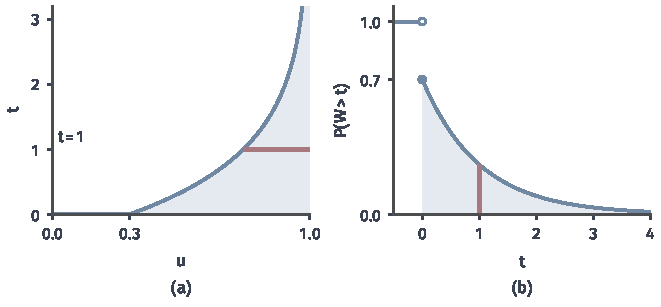
\includegraphics[width=112mm]{figures/07-probability/02-measure-theoretic-probability/matplotlib/pspace-tail-integral/figure.pdf}
  \caption{同一块面积的两种切法。(a)浅蓝区域在分位数函数$Q_W$的图像下方，红色横线是高度$t=1$处的切片，长度为$\mathbb{P}(W>1)=0.7\,\mathrm{e}^{-1}$；(b)蓝线是$\mathbb{P}(W>t)$，在$t=0$处从$1$降到$0.7$（实心点是函数值），红色竖线是同一个切片长度。两块浅蓝面积都等于$\mathbb{E}[W]=0.7$。}
  \label{fig:pspace-tail-integral}
\end{BookInlineFigure}

取值于非负整数时，$\mathbb{P}(T>t)$在每个区间$[k-1,k)$上等于$\mathbb{P}(T\geq k)$，式~\eqref{eq:pspace-tail-integral}就回到前面的级数公式$\mathbb{E}[T]=\sum_k\mathbb{P}(T\geq k)$。

\paragraph{独立对象的乘积期望}
第~\ref{chap:random-vectors}章对独立变量使用了$\mathbb{E}[XY]=\mathbb{E}[X]\,\mathbb{E}[Y]$，以及$\mathbb{E}[\phi(X,Y)]$的累次积分公式，在密度情形把它们当作计算规则。由乘积分布与分布积分公式，现在可以一般地证明。

\begin{theorem}[独立对象的期望]
\label{thm:pspace-independent-expectation}
设$X,Y$分别取值于$(E_1,\mathcal{E}_1)$与$(E_2,\mathcal{E}_2)$，相互独立，$\phi:E_1\times E_2\to\mathbb{R}$可测。若$\phi\geq0$，或$\phi(X,Y)$可积，则
\begin{equation}
  \mathbb{E}\bigl[\phi(X,Y)\bigr]=\int_{E_1}\Bigl(\int_{E_2}\phi(x,y)\,P_Y(\mathrm{d}y)\Bigr)P_X(\mathrm{d}x).
  \label{eq:pspace-independent-iterated}
\end{equation}
特别地，若实值随机变量$X,Y$独立且都可积，则$XY$可积，并且
\begin{equation}
  \mathbb{E}[XY]=\mathbb{E}[X]\,\mathbb{E}[Y].
  \label{eq:pspace-independent-product}
\end{equation}
\end{theorem}

\begin{proof}
由分布积分公式，$\mathbb{E}[\phi(X,Y)]$等于$\phi$对$P_{(X,Y)}$的积分。由定理~\ref{thm:pspace-independence-product}，$P_{(X,Y)}=P_X\otimes P_Y$。$\phi\geq0$时用Tonelli定理化为累次积分，即得式~\eqref{eq:pspace-independent-iterated}；$\phi(X,Y)$可积时用Fubini定理。

对乘积，先取$\phi(x,y)=\lvert x\rvert\lvert y\rvert\geq0$，内层积分是$\lvert x\rvert\,\mathbb{E}[\lvert Y\rvert]$，于是
\[
  \mathbb{E}\bigl[\lvert XY\rvert\bigr]=\mathbb{E}\bigl[\lvert X\rvert\bigr]\,\mathbb{E}\bigl[\lvert Y\rvert\bigr]<\infty,
\]
$XY$可积。再取$\phi(x,y)=xy$，用Fubini定理，内层积分是$x\,\mathbb{E}[Y]$，外层再积分得到式~\eqref{eq:pspace-independent-product}。
\end{proof}

用第~\ref{sec:pspace-independence}节的独立对$X\sim\operatorname{Unif}(0,1)$、$Y\sim\operatorname{Exp}(1)$算两个例子。由式~\eqref{eq:pspace-independent-product}，
\[
  \mathbb{E}[XY]=\tfrac12\cdot1=\tfrac12 .
\]
对$\phi(x,y)=\mathrm{e}^{-xy}$，它不是乘积形式，只能用累次积分。先对$y$积分，
\[
  \int_0^{\infty}\mathrm{e}^{-xy}\,\mathrm{e}^{-y}\,\mathrm{d}y=\frac{1}{1+x},
\]
再对$x$在$[0,1]$上积分，
\[
  \mathbb{E}\bigl[\mathrm{e}^{-XY}\bigr]=\int_0^1\frac{\mathrm{d}x}{1+x}=\ln2\approx0.6931 .
\]
式~\eqref{eq:pspace-independent-product}只是独立的一个推论，反过来不成立：第~\ref{chap:random-vectors}章已经看到，$\mathbb{E}[XY]=\mathbb{E}[X]\,\mathbb{E}[Y]$只说明不相关，不能推出独立。

\paragraph{Cantor变量的均值与方差}
最后回到章首的Cantor变量$X$，它等于$\sum_{k\geq1}2D_k/3^{k}$，其中$D_k$是第~\ref{sec:pspace-independence}节的独立公平比特。它既没有概率表也没有密度，可是$X$是非负随机变量，期望有定义。由式~\eqref{eq:pspace-series-exchange}，
\[
  \mathbb{E}[X]=\sum_{k=1}^{\infty}\frac{2\,\mathbb{E}[D_k]}{3^{k}}=\sum_{k=1}^{\infty}\frac{1}{3^{k}}=\frac12 .
\]
这与对称性一致：把每个$D_k$换成$1-D_k$，$X$变成$1-X$，而独立公平比特在这一替换下联合分布不变，所以$X\overset{\mathrm{d}}{=}1-X$。

方差要用支配收敛。令$\varepsilon_k=2D_k-1$，它等概率地取$\pm1$，各$\varepsilon_k$相互独立。记部分和
\[
  S_n=\sum_{k=1}^{n}\frac{\varepsilon_k}{3^{k}},\qquad \lvert S_n\rvert\leq\sum_{k=1}^{\infty}\frac{1}{3^{k}}=\frac12,
\]
它处处收敛到$X-\frac12$。展开平方，
\[
  \mathbb{E}[S_n^{2}]=\sum_{k=1}^{n}\frac{\mathbb{E}[\varepsilon_k^{2}]}{9^{k}}+\sum_{j\neq k}\frac{\mathbb{E}[\varepsilon_j\varepsilon_k]}{3^{j+k}}=\sum_{k=1}^{n}\frac{1}{9^{k}},
\]
其中$\varepsilon_k^{2}=1$，而$j\neq k$时$\varepsilon_j$与$\varepsilon_k$独立、均值为零，由式~\eqref{eq:pspace-independent-product}，交叉项的期望为零。

$S_n^{2}\to(X-\frac12)^{2}$处处成立，且$S_n^{2}\leq\frac14$，常数$\frac14$可积。由支配收敛定理，
\[
  \operatorname{Var}(X)=\lim_{n\to\infty}\mathbb{E}[S_n^{2}]=\sum_{k=1}^{\infty}\frac{1}{9^{k}}=\frac{1/9}{1-1/9}=\frac18 .
\]
标准差$\sqrt{1/8}\approx0.354$。图~\ref{fig:pspace-cantor-mean}是$20000$个模拟样本的直方图，样本均值约$0.498$，样本方差约$0.1250$。质量全部在Cantor集附近的若干小段上，均值$1/2$本身却落在中间被挖去的空隙里，没有任何样本能取到它；这再次说明期望是质量的重心，不必是可能的取值。

\begin{BookInlineFigure}
  \centering
  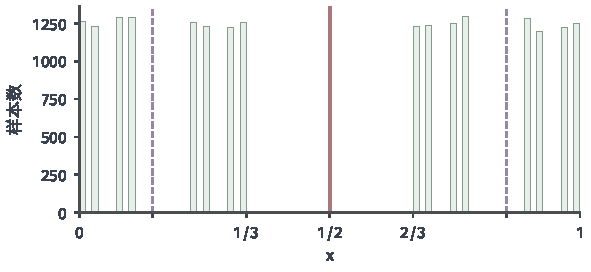
\includegraphics[width=100mm]{figures/07-probability/02-measure-theoretic-probability/matplotlib/pspace-cantor-mean/figure.pdf}
  \caption{Cantor变量的$20000$个模拟样本（每个样本保留$30$位三进制数字，种子$2026$），浅绿柱为$81$等分的直方图。红线是期望$1/2$，紫色虚线是$\frac12\pm\sqrt{1/8}$。样本都落在第二层保留的四段区间内，期望处于中间的空隙中。}
  \label{fig:pspace-cantor-mean}
\end{BookInlineFigure}

\paragraph{第一部分公式的来源}
表~\ref{tab:pspace-formula-sources}把第一部分的期望计算与它们在一般框架中的依据对应起来。每一行左边的公式，在第一部分只对概率表或密度验证过；右边的依据对任意分布都成立。

\begin{BookInlineTable}
  \centering
  \caption{第一部分的期望计算及其一般依据}
  \label{tab:pspace-formula-sources}
  \begin{tabular}{ll}
    \toprule
    第一部分的计算 & 一般框架中的依据 \\
    \midrule
    概率表求和$\sum_xg(x)p_X(x)$ & 分布积分公式，单点测度之和 \\
    密度积分$\int g(x)f_X(x)\,\mathrm{d}x$ & 分布积分公式，加权测度 \\
    混合分布分两部分计算 & 测度之和的积分 \\
    $\mathbb{E}[X+Y]=\mathbb{E}[X]+\mathbb{E}[Y]$ & 积分的线性 \\
    级数与期望交换 & 单调收敛、支配收敛 \\
    尾积分公式 & Tonelli定理 \\
    独立时$\mathbb{E}[XY]=\mathbb{E}[X]\,\mathbb{E}[Y]$ & 乘积分布与Fubini定理 \\
    \bottomrule
  \end{tabular}
\end{BookInlineTable}

\section{本章小结}
\label{sec:pspace-summary}

本章把第一部分分散的模型放进同一个框架。一个概率模型由三部分组成：样本空间$\Omega$列出可能的结果，事件族$\mathcal{F}$规定可以问概率的结果集合，概率测度$\mathbb{P}$给每个事件指定概率。事件族之所以要单独指定，是因为连续位置上无法给全部子集一致地赋予长度，也因为同一组结果在不同的观察者那里能回答的问题不同。它对补集和可数并封闭，因而是$\sigma$代数；在有限样本空间上，它就是一个划分及其各种并。

概率是总质量为一的测度。可数可加性推出概率沿单调事件列连续，由此得到分布函数的右连续性、两端极限和跳跃等于单点概率；分布函数又唯一确定实轴上的概率测度，任何满足三条性质的函数都对应一个分布，Cantor分布也在其中。单点概率为零与总概率为一并不矛盾，因为可加性只对可数个事件成立。零概率事件可以发生，几乎必然的陈述可以合并可数次，但不能合并不可数次；完备化把零概率事件的子集补为事件，使零概率修改不破坏可测性，却不改变任何原有概率，也不能使零概率条件变得可以相除。

随机对象是可测映射，可测性保证由观测引出的“取值落在某集合中”都是事件。实值、向量、矩阵和有限随机图都是它的特例，可测函数的复合仍是随机对象。观测生成的$\sigma$代数记录了它能区分的事件，对观测再作变换只会减少信息。随机对象的分布是概率在它下面的推前，变换后的分布由原像规则直接算出；分位数变换说明任何一维分布都可以由一个均匀随机点实现。处处相等、几乎必然相等与同分布依次减弱，边缘分布不能确定两个变量怎样配对，差与和的分布需要联合分布。

独立是信息族之间的乘法公式。它只需在对交封闭的生成族上检验，所以联合分布函数分解为乘积就足以推出独立；独立变量分组后的函数仍然独立。乘积测度造出了具有给定分布的独立对，独立等价于联合分布是边缘分布的乘积；木棍上一个均匀点的二进制数字是一列独立的公平比特，把这些数字拆组再作分位数变换，就得到具有任意分布的独立序列。

期望是随机变量对概率测度的积分：非负变量先用按取值分层的简单变量逼近，有符号变量再拆成正部与负部。线性、保序、单调收敛与支配收敛、分布积分公式、尾积分公式和独立乘积的期望，都是卷四积分理论的概率形式；第一部分的求和、密度积分和混合计算是它们的特例，等待时间的期望$0.7$与Cantor变量的方差$1/8$由此算出。

本章没有处理的是给定信息之后的平均。$\sigma(X)$描述了观测$X$提供的信息，下一章研究固定这部分信息、在每组已知结果内求平均得到的随机变量，即条件期望，并说明在观测值本身概率为零时怎样保留“组内平均”的含义。

